%%
%% abtex2-modelo-trabalho-academico.tex, v-1.9.2 laurocesar
%% Copyright 2012-2017 by abnTeX2 group at http://abntex2.googlecode.com/ 
%%
%% This work may be distributed and/or modified under the
%% conditions of the LaTeX Project Public License, either version 1.3
%% of this license or (at your option) any later version.
%% The latest version of this license is in
%%   http://www.latex-project.org/lppl.txt
%% and version 1.3 or later is part of all distributions of LaTeX
%% version 2005/12/01 or later.
%%
%% This work has the LPPL maintenance status `maintained'.
%% 
%% The Current Maintainer of this work is Emílio Eiji Kavamura,
%% eek.edu@outlook.com; emilio.kavamura@ufpr.br
%% Further information about abnTeX2 are available on 
%%
%% http://abntex2.googlecode.com/
%%
%% https://code.google.com/p/abntex2/issues/ 
%%
%% Further information about UFPR abnTeX2 are available on 
%%
%% https://github.com/eekBR/ufpr-abntex/
%%
%% This work consists of the files 
% 
%              main.tex   programa principal
%          00-dados.tex   entrada de dados 
%          00-pacotes.tex   pacotes carregados no modelo
% 00-pacotesOpcionais.tex   pacotes opcionais
      % 00-pretextual.tex   processamento dos elementos pre-textuais
%                UFPR.sty   ajusta do modelo canonico às normas  UFPR
%
%    referencias.bib
%                     e outras arquivos de imagens
%
%
%------------------------------------------------------------------------
% ------------------------------------------------------------------------
% abnTeX2: Modelo de Trabalho Academico (tese de doutorado, dissertacao de
% mestrado e trabalhos monograficos em geral) em conformidade com 
% ABNT NBR 6023:2018: Informação e documentação - Referências - Elaboração
% ------------------------------------------------------------------------
% ------------------------------------------------------------------------
%
% DATA DE ATUALIZAÇÃO: 2020-06-10

\documentclass[
        % -- opções da classe memoir --
        12pt,                           % tamanho da fonte
        openright,                      % capítulos começam em pág ímpar (insere página vazia caso preciso)
        %twoside,                        % para impressão em verso e anverso. Oposto a oneside
        oneside,
        a4paper,                        % tamanho do papel. 
        % -- opções da classe abntex2 --
        chapter=TITLE,         % títulos de capítulos convertidos em letras maiúsculas
        section=TITLE,         % títulos de seções convertidos em letras maiúsculas
        subsection=Title,      % títulos de subseções convertidos em letras maiúsculas
        %subsubsection=TITLE,  % títulos de subsubseções convertidos em letras maiúsculas
        % -- opções do pacote babel --
        english,                        % idioma adicional para hifenização
        %french,                         % idioma adicional para hifenização
        spanish,                        % idioma adicional para hifenização
        portugues,                      % o último idioma é o principal do documento
        %%%%%%%%%%%%
        %eek: colocação da opção para o sumario ter formatação tradicional
        %sumario=tradicional             % título no formato tradicional
        ]{abntex2}

\usepackage{UFPR}
% Pacotes básicos 
% ----------------------------------------------------------
%\usepackage{lmodern}			% Usa a fonte Latin Modern			
\usepackage[T1]{fontenc}		% Selecao de codigos de fonte.
\usepackage[utf8]{inputenc}		% Codificacao do documento (conversão automática dos acentos)
\usepackage{lastpage}			% Usado pela Ficha catalográfica
\usepackage{indentfirst}		% Indenta o primeiro parágrafo de cada seção.
\usepackage{microtype} 			% para melhorias de justificação
\usepackage{ifthen}		    	% para montar condicionais
\usepackage[brazil]{babel}		% para utilizar termos em portugues
\usepackage[final]{pdfpages}    % para incluir páginas de arquivos pdf
\usepackage{amsmath}			% simbolos matematicos
\usepackage{amsfonts}

% \usepackage{lstlistings}			% para listagem de codigos
% \usepackage[vlined,portuguese,onelanguage,algochapter]{algorithm2e}

% Pacotes de citações BibLaTeX
% ----------------------------------------------------------
\usepackage[style=abnt,
	backref=true,
	backend=biber,
	citecounter=true,
	backrefstyle=three, 
 	repeatfields=true,
	url=true,
	maxbibnames=99,
    mincitenames=1,
    maxcitenames=2,
    backref=true,
    hyperref=true,
    giveninits=true,
    uniquename=false,
    uniquelist=false,
	natbib=true]{biblatex}

% Norma NBR10.520/2023 - Sobrenomes em minúsculas
\renewcommand*{\mkbibnamefamily}[1]{#1}%

% Espaçamento entre os itens nas referências (espço de uma linha simples)
% ----------------------------------------------------------
\setlength\bibitemsep{\baselineskip}

% Texto padrão para as referências
% ----------------------------------------------------------
\DefineBibliographyStrings{brazil}{%
	 backrefpage  = {Citado \arabic{citecounter} vez na página},		% originally "cited on page"
	 backrefpages = {Citado \arabic{citecounter} vezes nas páginas},	% originally "cited on pages"
	 urlfrom      = {Dispon\'ivel em},
}

% Ajusta indentação de Referencias no ToC
% ----------------------------------------------------------
\defbibheading{bay}[\bibname]{%
  \chapter*{#1}%
  \markboth{#1}{#1}%
  \addcontentsline{toc}{chapter}
  %{\protect\numberline{}\bibname}
  {\bibname}
}

% Formatando o avançao dos títulos no sumário 
% ----------------------------------------------------------
\makeatletter
	\pretocmd{\chapter}{\addtocontents{toc}{\protect\addvspace{-12\p@}}}{}{}
	\pretocmd{\section}{\addtocontents{toc}{\protect\addvspace{-3\p@}}}{}{}
\makeatother

% https://groups.google.com/g/abntex2/c/ZYwE4t9uTFM
\makeatletter
\let\oldcontentsline\contentsline
\def\contentsline#1#2{%
	\expandafter\ifx\csname l@#1\endcsname\l@section
	\expandafter\@firstoftwo
	\else
	\expandafter\@secondoftwo
	\fi
	{%
		\oldcontentsline{#1}{\MakeTextUppercase{#2}}%
	}{%
		\oldcontentsline{#1}{#2}%
	}%
}
\makeatother

% Para retirar os símbolos <> da URL  
% ----------------------------------------------------------
\DeclareFieldFormat{illustrated}{\addspace #1\isdot}%
%\DeclareFieldFormat{url}{\bibstring{urlform}\addcolon\addspace<\url{#1}>}%
%\DeclareFieldFormat{url}{\bibstring{urlfrom}\addcolon\addspace<\url{#1}>}%
\DeclareFieldFormat{url}{\bibstring{urlfrom}\addcolon \space\addspace{#1}} 
% remove <> em urls de acordo com abnt-6023:2018	

% Ajustar o espaço para a formatação da data
% ----------------------------------------------------------
\DeclareFieldFormat{urldate}{\bibstring{urlseen}\addcolon\addspace #1}%
\DeclareFieldFormat*{note}{\addspace #1}%

% Para ajustar o tamanho da fonte do número da primeira página do capítulo
% comando utilizado na parte textual 
% ----------------------------------------------------------
\makepagestyle{chapfirst}% Just for the first page of a chapter
\makeoddhead{chapfirst}{}{}{\footnotesize{\thepage}}

%%criar um novo estilo de cabeçalhos e rodapés
\makepagestyle{simplestextual}
  %%cabeçalhos
  \makeevenhead{simplestextual} %%pagina par
     {}{}{\footnotesize \thepage}
     
  \makeoddhead{simplestextual} %%pagina ímpar ou com oneside
     {}{}{\footnotesize \thepage}
  %\makeheadrule{simplestextual}{\textwidth}{\normalrulethickness} %linha
  %% rodapé
  \makeevenfoot{simplestextual}
     {}{}{} %%pagina par
      
  \makeoddfoot{simplestextual} %%pagina ímpar ou com oneside
     {}{}{}
     
% Define a formatação dos capítulos póstextuais numerados
% ----------------------------------------------------------
%\newcommand{\refap}[1]{\hyperref[#1]{Apêndice~\ref{#1}}} 	% Referência apÊndices



 %%%%%%%%%%% NBR 10520/23

 % Norma NBR10.520/2023 - Sobrenomes em minúsculas
\renewcommand*{\mkbibnamefamily}[1]{#1}%

%fullcite com todos autores e não como cite
\makeatletter
\newcommand{\tempmaxup}[1]{\def\blx@maxcitenames{99}#1}
\makeatother

\DeclareCiteCommand{\fullcite}[\tempmaxup]
{\usebibmacro{prenote}}
{\usedriver
	{}
	{\thefield{entrytype}}}
{\multicitedelim}
{\usebibmacro{postnote}}


% \SetKwIF{Se}{SenaoSe}{Senao}{se}{então}{senão se}{senão}{fim-se}%
% \SetKwFor{Para}{para}{faça}{fim para}%
\usepackage{color}		    	% Controle das cores
\usepackage{graphicx}			% Inclusão de gráficos
\usepackage{lipsum}				% para geração de dummy text
\usepackage{csquotes}

%\usepackage[style=long]{glossaries}
%\usepackage{abntex2glossaries}

\usepackage{cancel} 		% permite representar o cancelamento de termos em texto ou equacoes	
\usepackage{xcolor} 		% cores extendidas	
\usepackage{smartdiagram}   	% gera diagramas a partir de listas
%\usepackage{float} 		% Para a figura ficar na posição correta	    
\usepackage{textcomp} 		% supporte para fontes da Text Companion 
\usepackage{longtable}		% uso de longtable

\usepackage{lscape}		% páginas em paisagem
\usepackage{multicol}		% mescla de colunas em tabelas
\usepackage{multirow}		% mescla de linhas em tabelas
\usepackage{newfloat} 		% criação do indice de quadros

\usepackage{mathtools}
\mathtoolsset{showonlyrefs}

\newcommand{\vetor}[1]{\ensuremath{{\vec{#1}}}}

%\usepackage{caption} 		% configura legenda 
%[format=plain]
%\renewcommand\caption[1]{%
	%\captionsetup{font=small}	% tamanho da fonte 10pt
	%,format=hang
	% \caption{#1}}
%\captionsetup{width=0.8\textwidth}
\captiondelim{-- }
\captiontitlefont{\small}
\captionnamefont{\small}


% uso do tikz e pgfplots
% ----------------------------------------------------------
%\usetikzlibrary{external}
\usetikzlibrary{arrows,calc,patterns,angles,quotes}
\usepackage{pgfplots}
\pgfplotsset{compat=1.15}


% Define o comando para citação de fontes em elementos gráficos (figuras, imagens,...).
% ----------------------------------------------------------
%  AUTOR(ano)
%
% parâmetro é a bibkey da fonte

\newcommand{\citefig}[2]{~\Citeauthor*{#1}\citeyear{#1}}

% Define os operadores matemáticos em portugues
% ----------------------------------------------------------
%

\DeclareMathOperator{\tr}{tr}
\DeclareMathOperator{\sen}{sen}
\DeclareMathOperator{\senh}{senh}
%\DeclareMathOperator{\tag}{tag}
\DeclareMathOperator{\tg}{tg}
\DeclareMathOperator{\tagh}{tagh}
\DeclareMathOperator{\tgh}{tgh}
\DeclareMathOperator{\cossec}{cossec}
%\DeclareMathOperator{\sen}{sen}

% Para fazer a listagem de codigos LaTeX na documentação
% ----------------------------------------------------------
\usepackage{listings}

% Comando para fazer 
%    a citação de documentos não publicados e informais e 
%    colocar as referências nas notas de rodapé
% ----------------------------------------------------------

\newcommand{\citenp}[1]{
	\cite{#1}\footnote{\fullcite{#1}}}

\newcommand{\textcitenp}[1]{
	\textcite{#1}\footnote{\fullcite{#1}}}


% para comentarios e sugestões
% ----------------------------------------------------------
\newcommand{\sugest}[1]{\textcolor{red!40}{#1}}


% simplificação para colocar figuras
% ----------------------------------------------------------
%   Parametros
%    1 caption
%    2 percent textwidth
%    3 arquivo da figura
%    4 fonte
%    5 fig:label
%    6 nota
%    7 legenda

\newcommand{\figura}[7]{
  {\centering
   \footnotesize
   \begin{figure}[!ht]
   \centering
        \caption{\uppercase{#1}}
        \includegraphics[width=#2\textwidth]{#3}
        \label{fig:#5}
    
    %ajustado p/ a largura da imagem
    \begin{minipage}{#2\textwidth} 
        \vspace{2mm}\centering
        %\begin{flushleft}
            \par FONTE:~#4
            \ifthenelse{\equal{#6}{}}{}
            { \par\hangindent=14mm NOTA: #6 }
            
            \ifthenelse{\equal{#7}{}}{}
            { \par\hangindent=14mm LEGENDA: #7 }
        %\end{flushleft}
    \end{minipage}
    \end{figure}
    }
}


% simplificação para colocar figuras cortadas
% ----------------------------------------------------------
%   Parametros
%    1 caption
%    2 percent textwidth
%    3 arquivo da figura
%    4 fonte
%    5 fig:label
%    6 nota
%    7 legenda
%    8 recorte esquerda direita em mm
%    9 recorte inferior superior em mm

\newcommand{\figurac}[9]{
 \centering\footnotesize
    \begin{figure}[!ht]
    {\centering
        \caption{\uppercase{#1}}
        \includegraphics[width=#2\textwidth, trim={#8mm #9 #8 #9},clip]{#3}
        \label{fig:#5}
        
    %ajustado p/ a largura da imagem
    \begin{minipage}{#2\textwidth} 
        \vspace{2mm}\centering
        %\begin{flushleft}
            \par FONTE:~#4
            \ifthenelse{\equal{#6}{}}{}
            {\par \hangindent=14mm NOTA: #6 }
          
            \ifthenelse{\equal{#7}{}}{}
            {\par \hangindent=14mm   LEGENDA: #7 }
        %\end{flushleft}
    \end{minipage}
    }
    \end{figure}
 
}

% simplificação para colocar imagens
% ----------------------------------------------------------
%   Parametros
%    1 caption
%    2 tabela
%    3 fonte
%    4 tab:label
%    5 nota
%    6 legenda

\newsavebox{\myboxa}
\newlength{\myboxlena}

\newcommand{\imagem}[6]{
	{
	\centering\footnotesize
  	    \sbox{\myboxa}{#2}
		\settowidth{\myboxlena}{\usebox{\myboxa}}
		\noindent
		\begin{figure}[!ht]
			\centering
			\caption{\uppercase{#1}}
			#2
			\label{fig:#4}
			
			%ajustado p/ a largura da imagem
			\begin{minipage}{\myboxlena} \footnotesize
				\vspace{2mm}\centering
				%\begin{flushleft}
				\par FONTE:~#3
				\ifthenelse{\equal{#5}{}}{}
				{ \par\hangindent=14mm NOTA: #5 }
				
				\ifthenelse{\equal{#6}{}}{}
				{ \par\hangindent=14mm LEGENDA: #6 }
				%\end{flushleft}
			\end{minipage}
		\end{figure}
	}
}

% simplificação para colocar tabelas
% ----------------------------------------------------------
%   Parametros
%    1 caption
%    2 tabela
%    3 fonte
%    4 tab:label
%    5 nota
%    6 legenda

\newsavebox{\mybox}
\newlength{\myboxlen}

\newcommand{\tabela}[6]
{
  \sbox{\mybox}{#2}
  \settowidth{\myboxlen}{\usebox{\mybox}}
  \noindent
  %\rule{\myboxlen}{1pt}\\
  \begin{table}[!ht]
    \centering\footnotesize
    \par\caption{\uppercase{#1}}
    
    \par  #2
 
    \label{tab:#4}
 
     \begin{minipage}{\myboxlen} 
        \vspace{2mm}\footnotesize
        %\begin{flushleft}
            FONTE:~ #3
            
            \ifthenelse{\equal{#5}{}}{}
            {\hangindent=14mm NOTA: #5 }
            
            \ifthenelse{\equal{#6}{}}{}
            {\hangindent=14mm LEGENDA: #6}
        %\end{flushleft}
    \end{minipage}
\end{table}
  % \centering
  % \usebox{\mybox}
  % box size: \the\myboxlen.
}

% Ambiente e lista de quadros
% ----------------------------------------------------------
\newfloat{quadro}{quadros}{QUADRO}
\newlistof{listofquadros}{quadros}{Lista de Quadros}
\newlistentry{quadro}{quadros}{0}
\cftsetindents{quadro}{0mm}{13mm}

%\PrepareListOf{quadro}{%
\renewcommand{\cftquadropresnum}{\normalsize{QUADRO}~}
\setlength{\cftquadronumwidth}{28mm}
%\renewcommand{\cftquadroname}{\quadroname\space} 
\renewcommand*{\cftquadroaftersnum}{\hfill--\hfill}
%}

\newsavebox{\myboxq}
\newlength{\myboxlenq}

% ----------------------------------------------------------
%   Parametros
%    1 caption
%    2 tabela/quadro
%    3 fonte
%    4 qua:label
%    5 nota
%    6 legenda

\newcommand{\qquadro}[6]
  {
   
   %\begin{center}
   \sbox{\myboxq}{#2}
   \settowidth{\myboxlenq}{\usebox{\myboxq}}
   \begin{quadro} \footnotesize
        \caption{\uppercase{#1}}
	\label{qua:#4}
        \noindent 
        
        #2 %placed inside the environment
	
   			
        %ajustado p/ a largura da tabela (quadro) se menor que 30mm a largura é ajustada para .5\linewidth
	 
        \ifdimcomp {\myboxlenq}{<}{30mm}{\settowidth{\myboxlenq}{\hspace{.5\linewidth}}}{}
    	
	\begin{minipage}{\myboxlenq} \footnotesize
    	    \vspace{2mm}\centering
    		%\begin{flushleft}
    		\par FONTE:~#3
    		\ifthenelse{\equal{#5}{}}{}
    		{ \par\hangindent=14mm NOTA: #5 }
    				
    		\ifthenelse{\equal{#6}{}}{}
    		{ \par\hangindent=14mm LEGENDA: #6 }
    		%\end{flushleft}
    	\end{minipage}
    %\end{center}
    \label{qua:#4}
  \end{quadro}
  } 

%%%%%%%%%%%%%%%%%%%%%%%%%%%%%%%%%%%%%%%%%%%%%%%%%%%%%%%
% Arquivo para entrada de dados para a parte pré textual
%%%%%%%%%%%%%%%%%%%%%%%%%%%%%%%%%%%%%%%%%%%%%%%%%%%%%%%
% 
% Basta digitar as informações indicidas, no formato 
% apresentado.
%
%%%%%%%
% Os dados solicitados são, na ordem:
%
% tipo do trabalho
% componentes do trabalho 
% título do trabalho
% nome do autor
% local 
% data (ano com 4 dígitos)
% orientador(a)
% coorientador(a)(as)(es)
% arquivo com dados bibliográficos
% instituição
% setor
% programa de pós gradução
% curso
% preambulo
% data defesa
% CDU
% errata
% assinaturas - termo de aprovação
% resumos & palavras chave
% agradecimentos
% dedicatoria
% epígrafe


% Informações de dados para CAPA e FOLHA DE ROSTO
%----------------------------------------------------------------------------- 
\tipotrabalho{Trabalho Acadêmico}
%    {Relatório Técnico}
%    {Dissertação}
%    {Tese}
%    {Monografia}

% Marcar Sim para as partes que irão compor o documento pdf
%----------------------------------------------------------------------------- 
 \providecommand{\terCapa}{Sim}
 \providecommand{\terFolhaRosto}{Sim}
 \providecommand{\terTermoAprovacao}{Nao}
 \providecommand{\terDedicatoria}{Nao}
 \providecommand{\terFichaCatalografica}{Nao}
 \providecommand{\terEpigrafe}{Nao}
 \providecommand{\terAgradecimentos}{Nao}
 \providecommand{\terErrata}{Nao}
 \providecommand{\terListaFiguras}{Nao}
 \providecommand{\terListaQuadros}{Nao}
 \providecommand{\terListaTabelas}{Nao}
 \providecommand{\terSiglasAbrev}{Nao} 
 \providecommand{\terSimbolos}{Nao}
 \providecommand{\terResumos}{Sim}            
 \providecommand{\terSumario}{Sim}
 \providecommand{\terAnexo}{Nao}
 \providecommand{\terApendice}{Nao}
 \providecommand{\terIndiceR}{Nao}
%----------------------------------------------------------------------------- 

\titulo{\textit{Splines} para Representação de Características Faciais com Aplicação em Biometria}
\autor{Maria Luiza Sampaio Logrado}
\local{Curitiba}
\data{2025} %Apenas ano 4 dígitos

% Orientador ou Orientadora
\orientador{
Prof Thiago de Oliveira Quinelato, DSc.}

% ----------------------------------------------------------
\addbibresource{referencias.bib}

% ----------------------------------------------------------
\instituicao{%
Universidade Federal do Paraná}

\preambulo{
Trabalho apresentado como requisito parcial à coclusão do curso de graduação em Matemática Industrial no Setor de Exatas da Universidade Federal do Paraná}

%----------------------------------------------------------------------------- 

\newcommand{\imprimirCurso}{}
%Programa de P\'os Gradua\c{c}\~ao em Engenharia da Constru\c{c}\~ao Civil}

\newcommand{\imprimirDataDefesa}{
09 de Dezembro de 2018}

\newcommand{\imprimircdu}{
02:141:005.7}

% ----------------------------------------------------------
\newcommand{\imprimirerrata}{
Elemento opcional da \cites[4.2.1.2]{NBR14724:2011}. Exemplo:

\vspace{\onelineskip}

FERRIGNO, C. R. A. \textbf{Tratamento de neoplasias ósseas apendiculares com
reimplantação de enxerto ósseo autólogo autoclavado associado ao plasma
rico em plaquetas}: estudo crítico na cirurgia de preservação de membro em
cães. 2011. 128 f. Tese (Livre-Docência) - Faculdade de Medicina Veterinária e
Zootecnia, Universidade de São Paulo, São Paulo, 2011.

\begin{table}[htb]
\center
\footnotesize
\begin{tabular}{|p{1.4cm}|p{1cm}|p{3cm}|p{3cm}|}
  \hline
   \textbf{Folha} & \textbf{Linha}  & \textbf{Onde se lê}  & \textbf{Leia-se}  \\
    \hline
    1 & 10 & auto-conclavo & autoconclavo\\
   \hline
\end{tabular}
\end{table}}

% Comandos de dados - Data da apresentação
\providecommand{\imprimirdataapresentacaoRotulo}{}
\providecommand{\imprimirdataapresentacao}{}
\newcommand{\dataapresentacao}[2][\dataapresentacaoname]{\renewcommand{\dataapresentacao}{#2}}

% Comandos de dados - Nome do Curso
\providecommand{\imprimirnomedocursoRotulo}{}
\providecommand{\imprimirnomedocurso}{}
\newcommand{\nomedocurso}[2][\nomedocursoname]
  {\renewcommand{\imprimirnomedocursoRotulo}{#1}
\renewcommand{\imprimirnomedocurso}{#2}}


% ----------------------------------------------------------
\newcommand{\AssinaAprovacao}{

\assinatura{%\textbf
   {Professora} \\ UFPR}
   \assinatura{%\textbf
   {Professora} \\ ENSEADE}
   \assinatura{%\textbf
   {Professora} \\ TIT}
   %\assinatura{%\textbf{Professor} \\ Convidado 4}
      
   \begin{center}
    \vspace*{0.5cm}
    %{\large\imprimirlocal}
    %\par
    %{\large\imprimirdata}
    \imprimirlocal, \imprimirDataDefesa.
    \vspace*{1cm}
  \end{center}
  }
  
% ----------------------------------------------------------
%\newcommand{\Errata}{%\color{blue}
%Elemento opcional da \textcite[4.2.1.2]{NBR14724:2011}. Exemplo:
%}

% ----------------------------------------------------------
\newcommand{\EpigrafeTexto}{%\color{blue}
\textit{``Não vos amoldeis às estruturas deste mundo, \\
		mas transformai-vos pela renovação da mente, \\
		a fim de distinguir qual é a vontade de Deus: \\
		o que é bom, o que Lhe é agradável, o que é perfeito.\\
		(Bíblia Sagrada, Romanos 12, 2)}
}

% ----------------------------------------------------------
\newcommand{\ResumoTexto}{%\color{blue}
O resumo deve ressaltar o  objetivo, o método, os resultados e as conclusões do documento. A ordem e a extensão destes itens dependem do tipo de resumo (informativo ou indicativo) e do tratamento que cada item recebe no documento original. O resumo deve ser precedido da referência do documento, com exceção do resumo inserido no próprio documento. (\ldots) As palavras-chave devem figurar logo abaixo do  resumo, antecedidas da expressão Palavras-chave:, separadas entre si por ponto e finalizadas também por ponto.Ter no máximo 500 palavras!!! As palavras chave são separadas por ponto e vírgula.
} 

\newcommand{\PalavraschaveTexto}{%\color{blue}
latex; abntex; editoração de texto.}

% ----------------------------------------------------------
\newcommand{\AbstractTexto}{%\color{blue}
This is the english abstract.
}
% ---
\newcommand{\KeywordsTexto}{%\color{blue}
latex. abntex. text editoration.
}

% ----------------------------------------------------------
\newcommand{\Resume}
{%\color{blue}
%Il s'agit d'un résumé en français.
} 
% ---
\newcommand{\Motscles}
{%\color{blue}
 %latex. abntex. publication de textes.
}

% ----------------------------------------------------------
\newcommand{\Resumen}
{%\color{blue}
%Este es el resumen en español.
}
% ---
\newcommand{\Palabrasclave}
{%\color{blue}
%latex. abntex. publicación de textos.
}

% ----------------------------------------------------------
\newcommand{\AgradecimentosTexto}{%\color{blue}
Os agradecimentos principais são direcionados à Gerald Weber, Miguel Frasson, Leslie H. Watter, Bruno Parente Lima, Flávio de  Vasconcellos Corrêa, Otavio Real Salvador, Renato Machnievscz\footnote{Os nomes dos integrantes do primeiro
projeto abn\TeX\ foram extraídos de \url{http://codigolivre.org.br/projects/abntex/}} e todos aqueles que contribuíram para que a produção de trabalhos acadêmicos conforme as normas ABNT com \LaTeX\ fosse possível.

Agradecimentos especiais são direcionados ao Centro de Pesquisa em Arquitetura da Informação\footnote{\url{http://www.cpai.unb.br/}} da Universidade de Brasília (CPAI), ao grupo de usuários
\emph{latex-br}\footnote{\url{http://groups.google.com/group/latex-br}} e aos novos voluntários do grupo \emph{\abnTeX}\footnote{\url{http://groups.google.com/group/abntex2} e
\url{http://abntex2.googlecode.com/}}~que contribuíram e que ainda
contribuirão para a evolução do \abnTeX.

Os agradecimentos principais são direcionados à Gerald Weber, Miguel Frasson, Leslie H. Watter, Bruno Parente Lima, Flávio de Vasconcellos Corrêa, Otavio Real Salvador, Renato Machnievscz\footnote{Os nomes dos integrantes do primeiro
projeto abn\TeX\ foram extraídos de \url{http://codigolivre.org.br/projects/abntex/}} e todos aqueles que contribuíram para que a produção de trabalhos acadêmicos conforme as normas ABNT com \LaTeX\ fosse possível.
}

% ----------------------------------------------------------
\newcommand{\DedicatoriaTexto}{%\color{blue}
\textit{ Dedico este trabalho a meus pais e seus respectivos cônjuges, \\
        que sempre me apoiaram e incentivaram durante essa jornada.}
	}



% compila o indice
% 
% ----------------------------------------------------------


\makeindex
% ----------------------------------------------------------
% Início do documento
% ----------------------------------------------------------
\begin{document}
% ----------------------------------------------------------
% Adequando o uppercase titulo dos elementos nas suas respectivas legendas
% Definicoes que n\~ao funcionaram quando colocados no arquivo de estilos ou de pacotes

\renewcommand{\bibname}{{REFER\^ENCIAS}}
\renewcommand{\tablename}{TABELA }
\renewcommand{\figurename}{FIGURA }
\renewcommand{\figureautorefname}{FIGURA}
\renewcommand{\tableautorefname}{TABELA}
\newcommand{\equationname}{equa\c{c}\~ao~}
\renewcommand{\equationautorefname}{equa\c{c}\~ao~}
\newcommand{\quadroautorefname}{QUADRO~}

% Para ajustar o tamanho da fonte do número da primeira página do capítulo
\aliaspagestyle{chapter}{chapfirst}% customizing chapter pagestyle

% ELEMENTOS PRÉ-TEXTUAIS
\makeoddhead{chapfirst}{}{}{}
% ----------------------------------------------------------
% Capa
% ----------------------------------------------------------
 \ifthenelse{\equal{\terCapa}{Sim}}{\imprimircapa}{}

% Folha de rosto
% ----------------------------------------------------------
\imprimirfolhaderosto*

% Inserir a ficha bibliografica
% ----------------------------------------------------------
 \ifthenelse{\equal{\terFichaCatalografica}{Sim}}
 {\insereFichaCatalografica{}\cleardoublepage}
 {}

% Inserir errata
% ----------------------------------------------------------
 \ifthenelse{\equal{\terErrata}{Sim}}
 {\begin{errata}%\color{blue}
   \imprimirerrata
  \end{errata}}
 {}

% Inserir folha de aprovação
% ----------------------------------------------------------
\ifthenelse{\equal{\terTermoAprovacao}{Sim}}{
\insereAprovacao}{}

% Dedicatória
% ----------------------------------------------------------
\ifthenelse{\equal{\terDedicatoria}{Sim}}{
\begin{dedicatoria}
   \vspace*{\fill}
   \centering
   \noindent
   \DedicatoriaTexto
   \vspace*{\fill}
\end{dedicatoria}
}{}

% Agradecimentos
% ----------------------------------------------------------

 \ifthenelse{\equal{\terAgradecimentos}{Sim}}
 {\begin{agradecimentos}
    \AgradecimentosTexto
  \end{agradecimentos}
  }{}
% Epígrafe
% ----------------------------------------------------------

\ifthenelse{\equal{\terEpigrafe}{Sim}}{
\begin{epigrafe}
    \vspace*{\fill}
	\begin{flushright}
        \EpigrafeTexto
	\end{flushright}
\end{epigrafe}
}{}

% RESUMOS
% ----------------------------------------------------------
% resumo em português
%\setlength{\absparsep}{18pt} % ajusta o espaçamento dos parágrafos do resumo
 \ifthenelse{\equal{\terResumos}{Sim}}{
\begin{resumo}
    \ResumoTexto
    
    %\vspace{\onelineskip}
    \noindent 
    \textbf{Palavras-chaves}: \PalavraschaveTexto
\end{resumo}

%% resumo em inglês
\begin{resumo}[ABSTRACT]
 \begin{otherlanguage*}{english}
   \AbstractTexto
   
   %\vspace{\onelineskip}
   \noindent 
   \textbf{Key-words}: \KeywordsTexto
 \end{otherlanguage*}
\end{resumo}


% resumo em francês 
\ifthenelse{\equal{\Resume}{}}
{}
{
 \begin{resumo}[RESUME]%Résumé
  \begin{otherlanguage*}{french}
     \Resume
     
     %\vspace{\onelineskip}
     \noindent      
     \textbf{Mots clés}: \Motscles
  \end{otherlanguage*}
 \end{resumo}
} 

% resumo em espanhol
\ifthenelse{\equal{\Resume}{}}{}
{ \begin{resumo}[RESUMEN]
  \begin{otherlanguage*}{spanish}
    \Resumen 
   
   %\vspace{\onelineskip}
   \noindent    
    \textbf{Palabras clave}: \Palabrasclave
  \end{otherlanguage*}
 \end{resumo}
}
}{}

% inserir lista de ilustrações
% ----------------------------------------------------------
\ifthenelse{\equal{\terListaFiguras}{Sim}}{
%\pdfbookmark[0]{\listfigurename}{lof}
\listoffigures*
\cleardoublepage
}{}

% inserir lista de quadros
% ----------------------------------------------------------
\ifthenelse{\equal{\terListaQuadros}{Sim}}{
%\pdfbookmark[0]{\listtablename}{lot}
\listofquadros*
\cleardoublepage
}{}

% inserir lista de tabelas
% ----------------------------------------------------------
\ifthenelse{\equal{\terListaTabelas}{Sim}}{
%\pdfbookmark[0]{\listtablename}{lot}
\listoftables*
\cleardoublepage
}{}



% inserir lista de abreviaturas e siglas 
% ----------------------------------------------------------

 \ifthenelse{\equal{\terSiglasAbrev}{Sim}}{
    \imprimirlistadesiglas
    \cleardoublepage
}{}


% inserir lista de símbolos
% ----------------------------------------------------------

 \ifthenelse{\equal{\terSimbolos}{Sim}}{
    \imprimirlistadesimbolos
    \cleardoublepage
 }{}

% inserir o sumario
\makeoddhead{chapfirst}{}{}{}
% ----------------------------------------------------------
\ifthenelse{\equal{\terSumario}{Sim}}{
%\pdfbookmark[0]{\contentsname}{toc}
\pagestyle{empty}
\tableofcontents*
\thispagestyle{empty}
%\cleardoublepage
}{}
 

 
 


% ----------------------------------------------------------
% ELEMENTOS TEXTUAIS
% ----------------------------------------------------------
\textual % \pagestyle{textualUFPR}

\pagestyle{simplestextual}
% sugerido por Youssef Cherem 20170316
% https://mail.google.com/mail/u/0/?tab=wm#inbox/15ad3fe6f4e5ff1f

% Introdução (exemplo de capítulo sem numeração, mas presente no Sumário)
% ----------------------------------------------------------
\chapter{INTRODUÇÃO} \label{cha:introd}

O reconhecimento facial é uma das áreas mais promissoras e desafiadoras dentro do campo da biometria. Sua aplicação abrange desde sistemas de segurança até autenticação em dispositivos móveis e portarias de condomínios, tornando-se cada vez mais presente no cotidiano. Nos últimos anos, métodos baseados em aprendizado profundo, especialmente redes neurais convolucionais (CNNs), têm dominado esse campo devido à sua alta acurácia. No entanto, tais métodos apresentam algumas limitações, especialmente no que diz respeito à interpretabilidade dos modelos e à necessidade de grandes volumes de dados para treinamento.

Nesse contexto, a busca por alternativas mais eficientes e interpretáveis tem ganhado relevância. Uma dessas alternativas é o uso de \textit{splines}, funções matemáticas capazes de gerar curvas suaves a partir de um conjunto reduzido de pontos. Ao representar as características faciais por meio de curvas, é possível reduzir significativamente a redundância dos dados, além de tornar o processo de extração e análise mais estruturado e compreensível.

Este trabalho propõe uma abordagem híbrida que combina a expressividade das \textit{splines} com técnicas de aprendizado de máquina para o reconhecimento facial. A metodologia baseia-se na extração de contornos das principais características do rosto, sua modelagem com \textit{splines} e posterior classificação utilizando algoritmos de comparação de sequências, como o \textit{Dynamic Time Warping} (DTW) \cite{SAKOE}. Espera-se, com isso, alcançar uma representação mais compacta e interpretável das feições faciais, sem comprometer o desempenho do sistema de identificação.

A introdução dessa nova abordagem se justifica não apenas pela busca por eficiência computacional, mas também pela necessidade de modelos que ofereçam maior transparência quanto às decisões tomadas. Dessa forma, o presente trabalho contribui para a ampliação das possibilidades de representação biométrica e propõe caminhos para o desenvolvimento de sistemas mais acessíveis, leves e explicáveis.

O método proposto para este trabalho foi implementado em Python e está disponível no repositório do GitHub \citep{MeuRepositorio}.


\section{OBJETIVO}

O objetivo deste trabalho é investigar a viabilidade do uso de \textit{splines} como método de representação de características faciais em sistemas biométricos, avaliando sua eficácia na melhoria do desempenho da identificação de indivíduos. A abordagem proposta visa combinar a expressividade das \textit{splines} com a capacidade do DTW para reconhecimento facial, buscando uma solução que seja ao mesmo tempo eficiente e interpretável.

\section{JUSTIFICATIVA}

Métodos convencionais baseados em CNNs e aprendizado profundo apresentam altos níveis de acurácia, mas muitos desses modelos operam como “caixas-pretas”, dificultando a interpretação das características extraídas e utilizadas para a tomada de decisão.

Diante desse cenário, a abordagem baseada no uso de \textit{splines} surge como uma alternativa para representação de características faciais de forma mais estruturada e interpretável. As \textit{splines} são funções matemáticas que permitem a modelagem de curvas suaves a partir de um conjunto reduzido de pontos de controle, garantindo uma representação eficiente das características faciais sem a necessidade de armazenar grandes quantidades de dados redundantes.

Além da compactação da informação, o uso de \textit{splines} facilita a extração de características relevantes, permitindo que apenas as estruturas mais significativas do rosto sejam utilizadas como entrada para o modelo de aprendizado. Isso pode melhorar a eficiência do DTW, aumentando a precisão na identificação.

Dessa forma, este trabalho se justifica pela necessidade de explorar métodos alternativos para reconhecimento facial que combinem eficiência computacional e interpretabilidade.

\section{METODOLOGIA}

A abordagem proposta para o reconhecimento facial baseada em \textit{splines} segue um fluxo estruturado, dividido em cinco etapas principais: detecção de características faciais, extração de contornos, redução de pontos, modelagem com \textit{splines} e classificação por DTW.

É importante esclarecer que a primeira versão das 4 primeiras etapas do método proposto neste trabalho foi desenvolvida durante o Programa de Voluntariado Acadêmico (PVA) em 2024 e neste TCC será desenvolvida a última etapa, que é a classificação por DTW, além de algumas melhorias nas etapas anteriores.

Por fim, trechos da pesquisa neste trabalho utilizam o banco de dados FERET \cite{FERET1,FERET2} de imagens faciais, coletado sob o programa FERET, patrocinado pelo Escritório do Programa de Desenvolvimento de Tecnologia Antidrogas do Departamento de Defesa dos EUA (DOD).

\subsection{Detecção de Características Faciais}

% Inicialmente, são identificadas as principais regiões do rosto, como olhos, boca e nariz. Para isso, é utilizado o modelo Haar Cascade \cite{BoostedCascade, HaarAplicacao} como a técnica de detecção. O modelo é ajustado para reconhecer padrões de características faciais em imagens, permitindo a localização das regiões de interesse.

Inicialmente, são identificadas as principais regiões do rosto, como olhos, boca e nariz. Para isso, é utilizado o modelo Haar Cascade \cite{BoostedCascade, HaarAplicacao} um algoritmo em cascata que utiliza métodos \textit{Boosting} para a detecção das características faciais.

\subsection{Extração de Contornos} 

Após a identificação das regiões faciais, são extraídos os contornos dessas características por meio da técnica de processamento de imagens de detecção de bordas utilizando o operador de Canny (segmentação baseada em gradientes para identificar regiões onde há mudanças bruscas de intensidade na imagem) \cite{Canny,CannyAplicacao}. O objetivo é obter um conjunto inicial de pontos que descrevem as características faciais.

% \subsection{Redução de Pontos}

% Para evitar redundância e reduzir a complexidade computacional, os pontos extraídos nos contornos são submetidos a um processo de simplificação. Estruturas de dados como grafos e árvore geradora mínima são utilizadas para manter apenas os pontos mais significativos. Nesta etapa utilizamos o algoritmo que encontra a árvore geradora mínima através da biblioteca \textit{Scipy} \cite{Scipy}.

% \subsection{Modelagem com \textit{splines}}

% Com os pontos reduzidos, são traçadas curvas suaves utilizando \textit{splines} Catmull-Rom \cite{CatmullRom, CatRomDemonstration, RepresentationSplines}. Essa modelagem permite representar as feições faciais de forma contínua e diferenciável, garantindo uma estrutura mais compacta e interpretável.

\subsection{Simplificação dos Contornos com Estruturas de Grafos}

Para reduzir a complexidade computacional, os pontos extraídos nos contornos são submetidos a um processo de simplificação. Estruturas de dados como grafos são utilizadas para armazenar os pontos e suas vizinhanças. A partir desses grafos, é possível aplicar algoritmos para identificação de seus componentes conexos \cite{Scipy}, mantendo aqueles que possuem os maiores números de nós, ou seja, os pontos mais significativos.

\subsection{Otimização Estrutural com Árvore Geradora Mínima}

Para garantir que as curvas não apresentem ciclos, é aplicada a técnica de árvore geradora mínima. Essa técnica permite selecionar um subconjunto de arestas que conecta todos os pontos sem formar ciclos, resultando em uma representação mais limpa e eficiente das características faciais. Após essa etapa, é implementado um algoritmo para encontrar o maior caminho entre os pontos e remover os pontos intermediários, resultando em uma curva mais simplificada.

\subsection{Classificação por \textit{Dynamic Time Warping}}

Por fim, os pontos gerados a partir dessas curvas são utilizados como entrada para um algoritmo de DTW \cite{SAKOE, tavenard.blog.dtw}. O DTW é um algoritmo que mede a similaridade entre duas sequências temporais, permitindo o alinhamento não-linear entre elas. Essa abordagem é especialmente útil para lidar com variações na velocidade e, neste trabalho, na forma das características faciais.

\section{REFERENCIAL TEÓRICO}

A ideia de representar características faciais por meio de \textit{splines} é discutida por \citet{RepresentationSplines}, que apresentam uma abordagem baseada em \textit{splines} Catmull-Rom para modelagem de curvas suaves. 

O uso do algoritmo de DTW para reconhecimento facial é abordado por \citet{DTW_LSTM}, que discutem a eficácia do DTW na comparação de sequências temporais, destacando sua aplicabilidade em tarefas de reconhecimento facial. No entanto, a abordagem proposta no artigo difere da adotada neste trabalho, uma vez que os autores concentram-se na análise das variações das cores dos pixels da imagem, em vez de explorar a forma ou a geometria das características faciais.

\section{CRONOGRAMA}

A Tabela \ref{tab:crono} apresenta o cronograma de atividades que foi planejado para o desenvolvimento do trabalho.

\begin{table}[ht] 
    \centering
    \caption{Cronograma de Atividades}
    \label{tab:crono}
    \begin{tabular}{|c|c|c|c|c|}
    \hline
    \textbf{Atividade} & \textbf{Mês 1} & \textbf{Mês 2} & \textbf{Mês 3} & \textbf{Mês 4} \\ \hline
    Refatoração do código & X &  &  & \\ \hline
    Revisão Bibliográfica &  X & X & X & X \\ \hline
    Estudo sobre \textit{Dynamic Time Warping} &  & X & X & \\ \hline
    Implementação do DTW &  & X & X & \\ \hline
    Escrita da Monografia & X & X & X & X \\ \hline
    Defesa do Trabalho &  &  &  &  X\\ \hline
    \end{tabular}
\end{table}


% PARTE DA PREPARAÇÃO DA PESQUISA
% ----------------------------------------------------------
%\part{Preparação da pesquisa}
\chapter{EXTRAÇÃO DE PONTOS DE FORMA AUTOMÁTICA} \label{cha:processamento-imagem} 

Neste capítulo será apresentado o método de extração automática de pontos, de forma a facilitar a modelagem de \textit{splines} para reconhecimento facial. O método proposto consiste em um algoritmo que utiliza técnicas de processamento de imagem e otimização para extrair pontos relevantes em imagens faciais. A abordagem é baseada na detecção de características faciais, seguida pela extração de contornos e filtragem dos pontos obtidos.

Inicialmente, realizamos uma pesquisa para identificar as principais características faciais a serem extraídas, decidindo focar na detecção dos olhos, nariz e boca. Para isso, utilizamos o algoritmo Haar Cascade \cite{BoostedCascade} para detectar o rosto da pessoa na imagem, concentrando a análise nessa área específica e facilitando a detecção das características menores.

Em seguida, utilizamos o método Canny do OpenCV \cite{CannyAplicacao, Canny} para extrair os contornos das características faciais. O Canny é um algoritmo de detecção de contornos eficiente que nos ajuda a identificar os limites das características faciais com maior precisão.

Após a extração dos contornos, suprimimos alguns pontos fazendo o uso de grafos e árvores geradoras mínimas. Essa etapa é crucial para reduzir a quantidade de pontos a serem utilizados na modelagem das \textit{splines}, mantendo apenas os pontos mais significativos que representam as características faciais. A simplificação dos pontos é realizada utilizando o algoritmo construído de forma autoral e implementado em Python, que utiliza a biblioteca \textit{Scipy} \cite{Scipy} para encontrar a árvore geradora mínima. Essa abordagem garante que os pontos extraídos sejam representativos e relevantes para a modelagem das \textit{splines}.

Por fim, ainda é possível aplicar um filtro de suavização para diminuir a quantidade de pontos, fazendo isso de forma completamente aleatória, mantendo apenas os pontos iniciais e finais de cada segmento, o que pode ser útil para melhorar a qualidade da modelagem das \textit{splines}.

\section{MODELOS PARA DETECÇÃO DE CARACTERÍSTICAS}

Foi utilizada uma abordagem popular de detecção chamada Haar Cascade, implementada com OpenCV e Python. Este método, introduzido e estudado no artigo \cite{BoostedCascade}, permite a detecção eficaz das características faciais.

O classificador Haar Cascade já foi calibrado e validado com um vasto conjunto de dados de rostos humanos, eliminando a necessidade de calibração adicional. Basta carregar o classificador da biblioteca e utilizá-lo para detectar rostos em uma imagem de entrada.

Para distinguir com precisão entre amostras que contêm ou não um rosto humano, utilizamos um classificador forte, resultante da combinação de diversos classificadores. Esta técnica envolve a utilização de uma cascata de classificadores para identificar diferentes características em uma imagem.

Os seguintes classificadores foram utilizados:

\begin{itemize}
    \item \texttt{haarcascade\_frontalface\_default.xml}
    \item \texttt{haarcascade\_eye.xml}
    \item \texttt{haarcascade\_mcs\_nose.xml}
    \item \texttt{haarcascade\_mcs\_mouth.xml}
\end{itemize}

Todos os classificadores mencionados podem ser encontrados no repositório do OpenCV no GitHub \cite{HaarAplicacao}.

\subsection{Parâmetros}

Após carregar os classificadores, podemos utilizá-los aplicando quatro parâmetros específicos para cada um.

O método \texttt{detectMultiScale()} é utilizado para identificar faces de diferentes tamanhos na imagem de entrada. Os quatro parâmetros principais deste método são detalhados a seguir:

\begin{itemize}
    \item \textbf{\texttt{image}}:
    \begin{itemize}
    \item O primeiro parâmetro é a imagem em tons de cinza, utilizada como entrada do método por facilitar a detecção das características faciais.
    \end{itemize}

\item \textbf{\texttt{scaleFactor}}:
\begin{itemize}
    \item Este parâmetro é usado para reduzir o tamanho da imagem de entrada, facilitando a detecção de faces maiores pelo algoritmo. Especificamos um fator de escala de 1.1, indicando que queremos reduzir o tamanho da imagem em 10\%.
    \end{itemize}

\item \textbf{\texttt{minNeighbors}}:
\begin{itemize}
    \item O classificador em cascata aplica uma janela deslizante através da imagem para detectar faces. Essas janelas são representadas como retângulos. Inicialmente, o classificador captura um grande número de falsos positivos. O parâmetro \texttt{minNeighbors} especifica o número de retângulos vizinhos que precisam ser identificados para que um objeto seja considerado uma detecção válida, ou seja, valores pequenos como 0 ou 1 resultam em muitos falsos positivos, enquanto valores grandes podem levar à perda de verdadeiros positivos. É necessário encontrar um equilíbrio que elimine falsos positivos e identifique com precisão os verdadeiros positivos.
\end{itemize}

\item \textbf{\texttt{minSize}}:
\begin{itemize}
    \item Este parâmetro define o tamanho mínimo do objeto a ser detectado. O modelo ignorará faces menores do que o tamanho mínimo especificado.
\end{itemize}

\end{itemize}

Foram colocados como \textit{default} para todos os classificadores os seguintes valores: 

{\small \texttt{detectMultiScale(image, scaleFactor=1.1, minNeighbors=5, minSize=(40, 50))}}

\subsection{Resultado da Detecção das Características}

Para realizar a detecção das características faciais, inicialmente identificamos o rosto na imagem. Esse processo retorna um \textit{array} com quatro valores: as coordenadas $x$ e $y$ do ponto onde o rosto foi detectado, além de sua largura e altura. Em seguida, recortamos a imagem nessa região, de modo a isolar a face da pessoa.

Com o rosto isolado, aplicamos classificadores específicos para detectar o nariz, a boca e os olhos.

Essa abordagem, que realiza a detecção passo a passo, garante maior precisão na identificação das características menores, pois concentra a análise na área previamente delimitada pelo rosto.

Considere a  \autoref{fig:deteccao-caracteristicas} , onde a detecção das características faciais é realizada:

\begin{enumerate}
\item \textbf{Detecção do Rosto:} Para identificar e isolar o rosto na imagem usamos o classificador \texttt{haarcascade\_frontalface\_default.xml}.
\item \textbf{Detecção dos Olhos:} Aplicamos o classificador \texttt{haarcascade\_eye.xml} para localizar os olhos dentro da área do rosto previamente detectada.
\item \textbf{Detecção do Nariz:} Utilizamos o classificador \texttt{haarcascade\_mcs\_nose.xml} para identificar o nariz na mesma área delimitada.
\item \textbf{Detecção da Boca:} Finalmente, aplicamos o classificador 

\texttt{haarcascade\_mcs\_mouth.xml} para localizar a boca.
\end{enumerate}

\begin{figure}[h!]
    \caption{DETECÇÕES.}
    \centering
    \begin{minipage}[b]{0.45\textwidth}
        \centering
        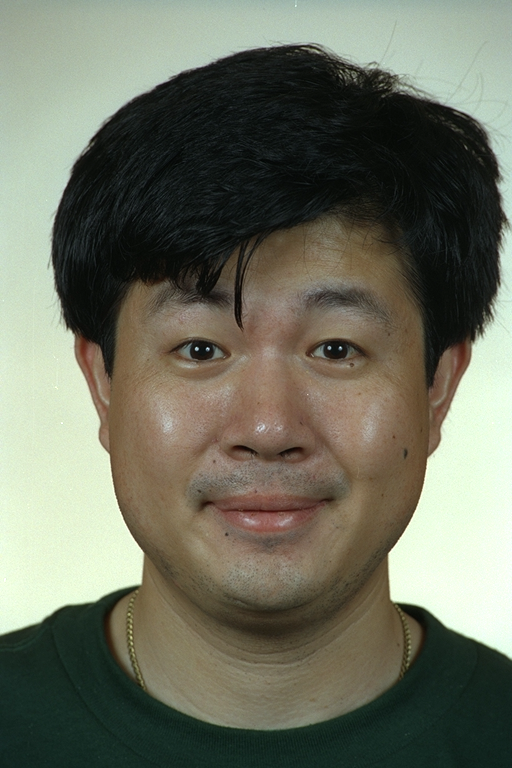
\includegraphics[width=0.9\linewidth]{fig/01_example_image.png}
        \legend{Imagem Original.}
        \label{fig:imagem}
    \end{minipage}
    \hfill
    \begin{minipage}[b]{0.45\textwidth}
        \centering
        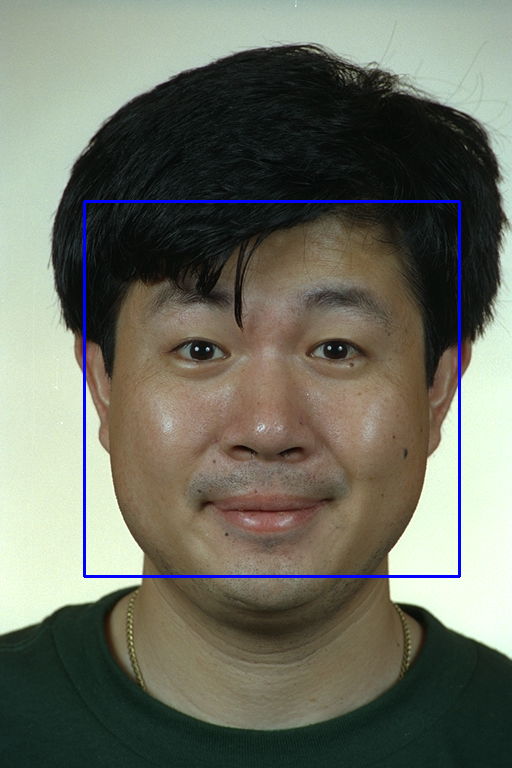
\includegraphics[width=0.9\linewidth]{fig/02_face.png}
        \legend{1º Detecção da face.}
        \label{fig:face}
    \end{minipage}

    \vspace{1cm}

    \begin{minipage}[b]{0.45\textwidth}
        \centering
        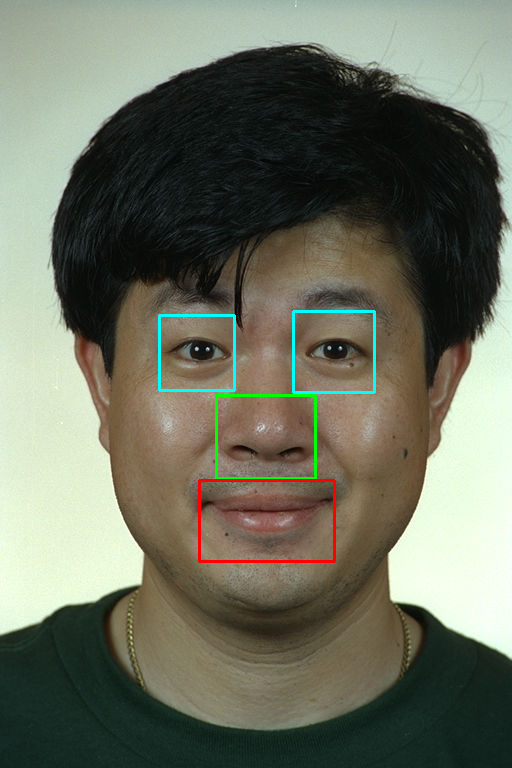
\includegraphics[width=0.9\linewidth]{fig/02_detected_features.png}
        \legend{2º Detecção das características.}
        \label{fig:caracteristicas}
    \end{minipage}
    \legend{FONTE: \cite{FERET1,FERET2}}
    \label{fig:deteccao-caracteristicas}
\end{figure}



\section{Extração de Contornos}

A detecção de contornos é essencial para a análise de imagens, pois permite a identificação de contornos e a segmentação de objetos em uma cena. O algoritmo de Canny \cite{Canny} é um dos métodos mais populares devido à sua eficiência e precisão. Esta seção irá explorar o funcionamento do algoritmo de Canny e demonstrará sua aplicação prática com a biblioteca OpenCV \cite{CannyAplicacao}.

\subsection{Algoritmo de Canny}

O algoritmo de detecção de contornos de Canny é composto por várias etapas, conforme descrito a seguir:

\begin{enumerate}
    \item \textbf{Redução de Ruído}: A imagem é suavizada com um filtro Gaussiano para minimizar a interferência do ruído na detecção de contornos.

    \item \textbf{Cálculo do Gradiente de Intensidade}: Os gradientes de intensidade da imagem são calculados nas direções horizontal e vertical, utilizando os operadores de Sobel. As componentes do gradiente são representadas por \( G_x = \frac{\partial I}{\partial x} \) e \( G_y = \frac{\partial I}{\partial y} \), onde \( I \) denota a imagem original. A magnitude do gradiente é então dada por:

    
    \[Contorno\_Gradiente(G) = \sqrt{G_{x}^{2} + G_{y}^{2}}\]

    \item \textbf{Supressão Não Máxima}: Elimina \textit{pixels} que não são máximos locais no gradiente, preservando apenas os que representam contornos fortes.

    \item \textbf{Rastreamento de Contornos por Histerese}: Classifica os contornos detectados usando dois limiares, \textit{minVal} e \textit{maxVal}:
    \begin{itemize}
        \item Contornos com gradiente maior que \textit{maxVal} são fortes.
        \item Contornos com gradiente menor que \textit{minVal} são descartados.
        \item Contornos entre \textit{minVal} e \textit{maxVal} são fracos e mantidos apenas se conectados a contornos fortes.
    \end{itemize}
\end{enumerate}

Por exemplo, na \autoref{fig:histerese}, o contorno A está acima do \textit{maxVal}, sendo assim considerado um contorno forte. Embora o contorno C esteja abaixo do \textit{maxVal}, ele está conectado ao contorno A, de modo que também é considerado como contorno válido, resultando em uma curva completa. Já o contorno B, embora esteja acima do \textit{minVal}, não está conectado a nenhum contorno forte e, portanto, é descartado.

\imagem{Rastreamento de contorno por histerese}{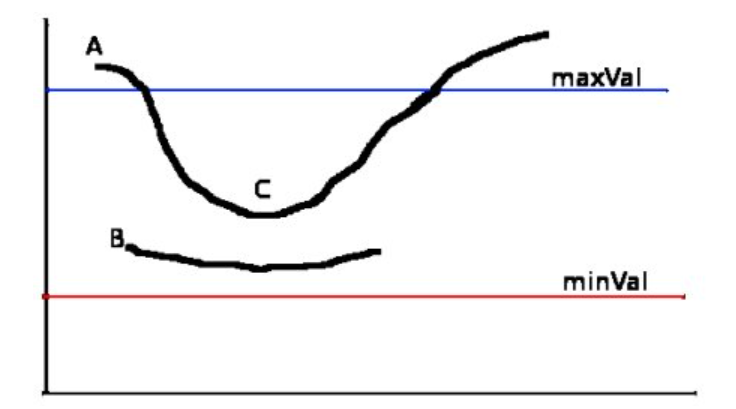
\includegraphics[width = 80mm]{fig/histerese}}{\cite{CannyAplicacao}}{histerese}{}{No eixo horizontal estão as curvas parametrizadas e no eixo vertical estão os valores de intensidade do gradiente.}

É crucial selecionar adequadamente os valores de \textit{minVal} e \textit{maxVal} para obter resultados precisos. Esse estágio também ajuda a remover pequenos ruídos de \textit{pixels}, assumindo que os contornos são linhas longas e contínuas.

\subsection{Resultado da Detecção de Contornos}
\label{sec:resultado-deteccao-contornos}

Ao aplicar o algoritmo de Canny para a detecção de contornos, obtemos um \textit{array} binário onde os valores `0' e `255' representam diferentes tipos de \textit{pixels}. Os \textit{pixels} com valor `0' são considerados descartáveis, ou seja, não fazem parte dos contornos detectados. Em contraste, os \textit{pixels} com valor `255' são os que definem os contornos, indicando regiões de mudança de intensidade significativa na imagem original.

A \autoref{fig:canny-contornos} ilustra a matriz Canny e os contornos resultantes.

\begin{figure}[ht]
    \caption{MATRIZ CANNY E CONTORNOS.}
    \label{fig:canny-contornos}
    \centering
    \begin{tabular}{c c c}
        \begin{minipage}{0.4\textwidth}
            \centering
            \textbf{Matriz Canny}\\ [0.2cm]
            \[
            \begin{bmatrix}
                255_1 & 0 & 0 & 0 & 0 \\
                0 & 255_2 & 0 & 255_3 & 0 \\
                255_4 & 0 & 0 & 0 & 255_5 \\
            \end{bmatrix}
            \]
        \end{minipage}
        \hspace{0.5cm}
        
        & $\rightarrow$ &
        \begin{minipage}{0.4\textwidth}
            \centering
            \textbf{Contornos}\\ [0.2cm]
            
\includegraphics[width=0.9\textwidth]{fig/contorno_canny.jpeg}
        \end{minipage}
    \end{tabular}
\end{figure}

A \autoref{fig:canny-aplicacao} apresentada os resultados da aplicação do algoritmo de Canny em imagens de características faciais.


\begin{figure}[h!]
    \caption{APLICAÇÃO DO ALGORITMO DE CANNY.}
    \centering
    \begin{minipage}[b]{0.45\textwidth}
        \centering
        
\includegraphics[width=0.9\linewidth]{fig/03_left_eye_edge.png}
        \legend{Olho esquerdo.}
        \label{fig:canny-esquerdo}
    \end{minipage}
    \hfill
    \begin{minipage}[b]{0.45\textwidth}
        \centering
        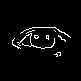
\includegraphics[width=0.9\linewidth]{fig/03_right_eye_edge.png}
        \legend{Olho direito.}
        \label{fig:canny-direito}
    \end{minipage}

    \vspace{1cm}

    \begin{minipage}[b]{0.45\textwidth}
        \centering
        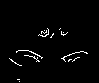
\includegraphics[width=0.9\linewidth]{fig/03_nose_edge.png}
        \legend{Nariz.}
        \label{fig:canny-nariz}
    \end{minipage}
    \hfill
    \begin{minipage}[b]{0.45\textwidth}
        \centering
        
\includegraphics[width=0.9\linewidth]{fig/03_mouth_edge.png}
        \legend{Boca.}
        \label{fig:canny-boca}
    \end{minipage}
    \label{fig:canny-aplicacao}
\end{figure}
% \newpage
Esses resultados demonstram como o algoritmo de Canny é eficaz para realçar os contornos em diferentes tipos de imagens, permitindo uma análise visual clara e detalhada das características principais em cada exemplo.

\newpage

\section{Redução de Pontos em Detecção de Contornos}
\label{sec:reduzindo-pontos-deteccao-contornos}


Embora o algoritmo de Canny seja excelente para capturar os contornos, nem sempre é necessário utilizar todos os pontos detectados ao passar uma \textit{spline}. Para a modelagem de contornos suaves e contínuos, é suficiente selecionar um subconjunto representativo dos pontos detectados. Esse processo pode envolver a amostragem ou a simplificação de alguns desses pontos, garantindo que a \textit{spline} mantenha a forma geral do contorno sem a complexidade de lidar com todos os pontos individuais.

Esta parte é realizada em cinco etapas principais:
\begin{enumerate}
    \item \textbf{Construção do Grafo:} Os pontos de contorno detectados são organizados em um grafo, onde cada ponto é um nó e as vizinhanças entre eles representam as arestas. Essa estrutura facilita a análise e a manipulação dos pontos.
    \item \textbf{Identificação de Componentes Conexos:} A partir do grafo, são identificados os componentes conexos, mantendo apenas os de maior tamanho. Isso é feito para garantir que apenas as partes mais significativas dos contornos sejam consideradas, eliminando ruídos e pontos irrelevantes.
    \item \textbf{Árvore Geradora Mínima:} A partir dos maiores componentes conexos, uma árvore geradora mínima é construída. Essa árvore conecta todos os pontos de forma a remover ciclos, resultando em uma representação mais limpa e eficiente dos contornos.
    \item \textbf{Otimização com Poda da Árvore:} A árvore geradora mínima é otimizada, removendo mais uma vez ruídos e mantendo apenas os pontos mais significativos.
    \item \textbf{Filtragem Aleatória:} Por fim, uma filtragem aleatória é aplicada para suavizar ainda mais a representação, mantendo apenas os pontos iniciais e finais de cada segmento. Essa etapa garante que a \textit{spline} resultante seja suave e contínua.
\end{enumerate}

\subsection{Grafos}

Para a construção do grafo, utilizamos os pontos de contorno detectados pelo algoritmo de Canny. Cada ponto é representado como um nó no grafo, e as vizinhanças entre os nós são representadas como arestas. Neste trabalho, a matriz de adjacências é utilizada para armazenar essas vizinhanças.

O código foi feito de forma autoral em Python, utilizando a fórmula Manhattan para calcular a distância entre os nós. Essa fórmula é adequada para o nosso caso, pois considera apenas as distâncias horizontais, verticais e diagonais, o que é suficiente para que o grafo represente adequadamente a estrutura dos contornos faciais.

Sejam os pontos \( i = (x_1, y_1) \) e \( j = (x_2, y_2) \). Definimos a distância Manhattan \( d(i, j) \) e a vizinhança \( v(i, j) \) como:

\begin{equation}
    \label{eq:distancia-manhattan}
    d(i, j) =
    \begin{cases}
    1, & \text{se } (x_1 = x_2 \lor y_1 = y_2) \text{ e } (x_1, y_1) \neq (x_2, y_2) \\
    2, & \text{se } |x_1 - x_2| = 1 \text{ e } |y_1 - y_2| = 1 \\
    \infty, & \text{caso contrário}
    \end{cases}
\end{equation}

\begin{equation}
    \label{eq:vizinhanca-manhattan}
    v(i, j) =
    \begin{cases}
    1, & \text{se } d(i, j) = 1 \text{ ou } d(i, j) = 2 \\
    0, & \text{caso contrário}
    \end{cases}
\end{equation}


A partir da matriz resultante da detecção de bordas por Canny (\autoref{fig:canny-contornos}), é possível construir a matriz de adjacências com base na distância de Manhattan (\ref{eq:distancia-manhattan}) e na definição de vizinhança adotada (\ref{eq:vizinhanca-manhattan}). Essa matriz representa, de forma matricial, as conexões entre os pixels considerados como nós do grafo, onde cada elemento \( a_{ij} \) indica a existência (ou não) de uma aresta entre os nós \( i \) e \( j \).

A \autoref{fig:adjacencias-grafo} ilustra tanto a matriz de adjacências quanto o grafo correspondente aos contornos identificados na \autoref{fig:canny-contornos}. Na matriz, cada linha e coluna correspondem a um nó, e os valores registrados indicam a presença ou ausência de conexões entre os pares de nós.


\begin{figure}[ht]
    \caption{MATRIZ DE ADJACÊNCIAS E GRAFO.}
    \label{fig:adjacencias-grafo}
    \centering
    \begin{tabular}{c c c}
        \begin{minipage}{0.4\textwidth}
            \textbf{Matriz de Adjacências}\\[0.2cm]
            \centering
            \[
            \begin{bmatrix}
                0 & 1 & 0 & 0 & 0 \\
                1 & 0 & 0 & 1 & 0 \\
                0 & 0 & 0 & 0 & 1 \\
                0 & 1 & 0 & 0 & 0 \\
                0 & 0 & 1 & 0 & 0 \\
            \end{bmatrix}
            \]
        \end{minipage}
        \hspace{0.5cm}
        
        & $\rightarrow$ &
        \begin{minipage}{0.4\textwidth}
            \centering
            \textbf{Grafo}\\[0.2cm]
                \begin{tikzpicture}[scale=1.2, every node/.style={circle, draw, minimum size=1cm}]
                    % Triângulo
                    \node [fill = blue!50, draw = blue] (1) at (2,1.5) {1};
                    \node [fill = blue!50, draw = blue] (2) at (4,1.5) {2};
                    \node [fill = blue!50, draw = blue] (4) at (3.5,0) {4};
                
                    % Conexão do nó 1 com nó 5 ao lado
                    \node [fill = red!50, draw = red](3) at (5.5, 1.5) {3};
                    \node [fill = red!50, draw = red](5) at (6,0) {5};
                
                    \draw (1) -- (2) -- (4);
                    \draw (3) -- (5);
                \end{tikzpicture}
        \end{minipage}
    \end{tabular}
    \end{figure}


\subsection{Grafos Conexos e Desconexos}

Os grafos podem ser classificados em dois tipos principais: grafos conexos e grafos desconexos. Um grafo é considerado conexo se existe pelo menos um caminho entre qualquer par de nós do grafo. Por outro lado, um grafo desconexo possui pelo menos um par de nós que não estão conectados por um caminho.

Um grafo desconexo pode ser dividido em componentes conexos, que são subgrafos conexos. Cada componente conexo é um subconjunto do grafo original onde há pelo menos um caminho conectando cada par de nós, mas não há conexão com os nós de outros componentes. Essa distinção é importante para entender a estrutura do grafo e como ele pode ser analisado e manipulado.


\begin{figure}[ht]
    \caption{COMPONENTES CONEXOS REPRESENTADOS POR GRAFOS.}
    \centering
    \begin{minipage}{0.45\textwidth}
        \centering
        \textbf{Componente Conexo 1} \\[0.2cm]
        \begin{tikzpicture}
            % Primeiro grafo (Triângulo) - Cor Azul
            \node at (2,1.5) (n1) [circle, draw=blue, fill=blue!50] {1};
            \node at (4,1.5) (n2) [circle, draw=blue, fill=blue!50] {2};
            \node at (3.5,0) (n3) [circle, draw=blue, fill=blue!50] {4};
            \draw (n1) -- (n2) -- (n3);
            % \draw (n2) -- (n3);
            % \draw (n3) -- (n1);
        \end{tikzpicture}
    \end{minipage}
    \hfill
    \begin{minipage}{0.45\textwidth}
        \centering
        \textbf{Componente Conexo 2} \\[0.2cm]
        \begin{tikzpicture}
            % Segundo grafo (Quadrado) - Cor Vermelha
            \node at (1.5,1.5) (n1) [circle, draw=red, fill=red!50] {3};
            \node at (2,0) (n2) [circle, draw=red, fill=red!50] {5};
            % \node at (2,2) (n3) [circle, draw=red, fill=red!50] {6};
            % \node at (0,2) (n4) [circle, draw=red, fill=red!50] {7};
            \draw (n1) -- (n2);
            % \draw (n2) -- (n3);
            % \draw (n3) -- (n4);
            % \draw (n4) -- (n1);
        \end{tikzpicture}
    \end{minipage}
    \label{fig:componentes_conexos}
    \end{figure}

% Em problemas de processamento de imagens, frequentemente são utilizados grafos que representam os \textit{pixels} da imagem. O objetivo é identificar componentes conexos, permitindo a seleção dos caminhos mais significativos e a filtragem de ruídos. Componentes com um grande número de nós indicam regiões de interesse, correspondendo a áreas com maior quantidade de \textit{pixels} conectados. Por outro lado, componentes menores podem ser interpretadas como ruído ou regiões irrelevantes, que podem ser descartadas durante o processamento.

 Nesta etapa do trabalho, o objetivo principal é reduzir ruídos nas imagens por meio da identificação de componentes conexas. Essa abordagem permite isolar regiões com alta densidade de \textit{pixels} conectados -- geralmente associadas a estruturas relevantes -- e descartar pequenas componentes, que tendem a representar ruído ou informações irrelevantes.


\subsection{Resultado da Construção do Grafo}
\label{sec:resultado-construcao-grafo}

Podemos observar que a imagem original é composta por um grande número de pontos, porém utilizando a filtragem de \textit{pixels} através de grafos com os maiores componentes conexos, conseguimos reduzir a quantidade de pontos, mantendo apenas os mais relevantes. A \autoref{fig:resultado-grafo} mostra o resultado da construção do grafo e a filtragem dos pontos.

\begin{figure}[h!]
    \caption{COMPONENTES CONEXOS OLHO DIREITO.}
    \centering
    \begin{minipage}[b]{0.45\textwidth}
        \centering
        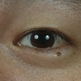
\includegraphics[width=0.9\linewidth]{fig/02_detected_right_eye.png}
        \legend{Olho direito identificado.}
        \label{fig:olho}
    \end{minipage}
    \hfill
    \begin{minipage}[b]{0.45\textwidth}
        \centering
        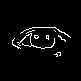
\includegraphics[width=0.9\linewidth]{fig/03_right_eye_edge.png}
        \legend{Ênfase nos contornos.}
        \label{fig:canny-olho}
    \end{minipage}

    \vspace{1cm}

    \begin{minipage}[b]{0.45\textwidth}
        \centering
        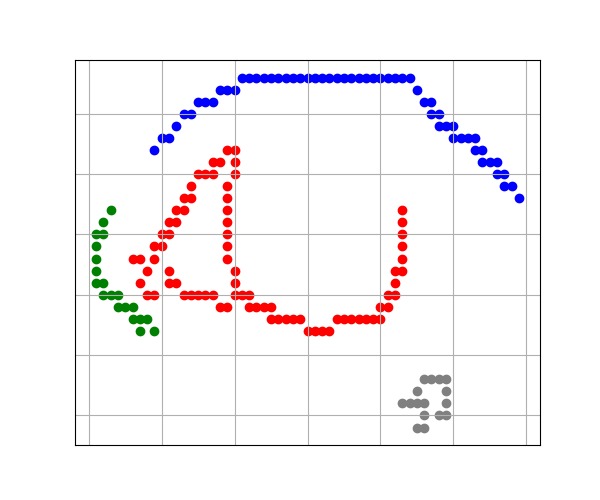
\includegraphics[width=1\linewidth]{fig/04_connected_components_right_eye.png}
        \legend{Remoção de alguns pontos através dos maiores compenentes conexos.}
        \label{fig:grafos-olho}
    \end{minipage}
    \label{fig:resultado-grafo}
\end{figure}

\subsection{Árvore Geradora Mínima}
\label{sec:arvore-geradora-minima}

A árvore geradora mínima (AGM) é uma estrutura de dados fundamental em teoria dos grafos, que conecta todos os nós de um grafo com o menor custo total possível. Essa estrutura é especialmente útil em aplicações de processamento de imagens, onde a simplificação de contornos e a redução do número de pontos são necessárias para facilitar a modelagem e a análise. Neste trabalho foi utilizada a biblioteca \textit{Scipy} \cite{Scipy} para encontrar a AGM.

Cada nó na AGM tem uma relação hierárquica com outros nós:

\begin{itemize}
    \item O nó raiz é o nó inicial a partir do qual a árvore é construída ou percorrida.
    \item Um nó filho é aquele que se origina de outro nó -- chamado de pai -- seguindo essa ideia de crescimento ou expansão da árvore.
    \item A folha é um nó que não tem filhos, ou seja, ela está no fim de um caminho na árvore
\end{itemize}

Para este trabalho, a AGM é utilizada para conectar os pontos de contorno detectados, formando uma estrutura que representa as características faciais de forma eficiente removendo ciclos. A \autoref{fig:arvore-geradora-minima} ilustra a Ávore Geradora Mínima construída entre os pontos de contorno, removendo os ciclos.

\begin{figure}
    \caption{ÁRVORE GERADORA MÍNIMA.}
    \label{fig:arvore-geradora-minima}
    \centering
    \begin{tikzpicture}[scale=1.5, every node/.style={circle, draw=gray!60, fill=gray!20, thick, minimum size=10mm}, 
    edge/.style={draw=black!70, thick},
    highlight/.style={draw=red, thick}]

    % Nodes
    \node (a) at (0,0) {c};
    \node (b) at (1.5,1.5) {d};
    \node (c) at (3,0) {e};
    \node (d) at (1.5,-1.2) {f};
    \node (e) at (-1.5,-1.2) {a};
    \node (f) at (-1.5,1.5) {b};

    % % Regular edges with weights
    \draw[edge] (a) -- (b);
    \draw[edge] (f) -- (e);
    \draw[edge] (b) -- (c);
    \draw[edge] (e) -- (d);
    \draw[edge] (c) -- (d);

    % Highlighted MST edges
    \draw[highlight] (f) -- (b);
    \draw[highlight] (f) -- (a);
    \draw[highlight] (a) -- (c);
    \draw[highlight] (a) -- (e);
    \draw[highlight] (a) -- (d);

    \end{tikzpicture}
    \legend{Em vermelho é destacado o caminho da AGM.}
\end{figure}

\subsection{Otimização da Árvore Geradora Mínima}

Para otimizar a análise, aplicamos uma poda da árvore na AGM para identificar o caminho principal e eliminar os pontos que não contribuem significativamente para a forma geral do contorno. Essa poda é realizada com base em critérios de comprimento e relevância, garantindo que apenas os pontos mais significativos sejam mantidos na representação final.


Veja abaixo a implementação do método \texttt{prunning\_tree}. Ele percorre recursivamente a árvore para calcular a altura dos nós e determinar o caminho de maior comprimento entre dois nós folha.

\begin{lstlisting}[language=Python, caption={IMPLEMENTAÇÃO DO MÉTODO \texttt{prunning\_tree}.}, label={lst:prunning_tree}]
def prunning_tree(self, raiz):
    # Se o nó atual não tem filhos, é uma folha
    if len(raiz.filhos) == 0:
        return 1, [raiz.idx], 1, [raiz.idx]
    else:
        # Para cada filho, executa a função recursivamente
        for filho in raiz.filhos:
            filho.altura, filho.caminho_altura_maxima, filho.tamanho_caminho_maximo, filho.caminho_maximo = self.prunning_tree(filho)

        if len(raiz.filhos) == 1:
            # Verifica se o caminho que passa pelo nó atual é maior que o maior caminho encontrado até o momento
            if raiz.filhos[0].altura + 1 > raiz.filhos[0].tamanho_caminho_maximo:
                tamanho_caminho_maximo = raiz.filhos[0].altura + 1
                caminho_maximo = [raiz.idx] + raiz.filhos[0].caminho_altura_maxima
            else:
                # Usa o maior caminho já encontrado no filho
                tamanho_caminho_maximo = raiz.filhos[0].tamanho_caminho_maximo
                caminho_maximo = raiz.filhos[0].caminho_maximo
        else:
            # Ordena os filhos pela altura (do maior para o menor)
            raiz.filhos.sort(key=lambda x: x.altura, reverse=True)

            # Calcula o maior caminho passando por este nó (soma das duas maiores alturas + o nó atual)
            tamanho_caminho_maximo = raiz.filhos[0].altura + raiz.filhos[1].altura + 1

            # Monta o caminho correspondente
            uma_parte_do_caminho = raiz.filhos[0].caminho_altura_maxima.copy()
            uma_parte_do_caminho.reverse()
            caminho_maximo = uma_parte_do_caminho + [raiz.idx] + raiz.filhos[1].caminho_altura_maxima

            # Verifica se algum filho tem um caminho maior do que esse
            for filho in raiz.filhos:
                if filho.tamanho_caminho_maximo > tamanho_caminho_maximo:
                    tamanho_caminho_maximo = filho.tamanho_caminho_maximo
                    caminho_maximo = filho.caminho_maximo

        # Pega o filho com maior altura (o primeiro da lista, já ordenada)
        no_altura_maxima = raiz.filhos[0]

        return no_altura_maxima.altura + 1, [raiz.idx] + no_altura_maxima.caminho_altura_maxima, tamanho_caminho_maximo, caminho_maximo

\end{lstlisting}

O funcionamento do algoritmo pode ser resumido nos seguintes passos:

\begin{enumerate}
    \item \textbf{Cálculo da Altura da Árvore} medindo a profundidade máxima a partir da raiz até as folhas.
    \item \textbf{Cálculo do Maior Caminho} dentro dos nós da árvore.
    \item O maior desses dois valores é considerado o \textbf{caminho principal}, capturando a estrutura mais relevante e eliminando nós de menor importância.
\end{enumerate}


\begin{figure}[ht]
    \centering
    \caption{PODA DA AGM.}
    \label{fig:poda-arvore-geradora-minima}
    \begin{tikzpicture}[
      level distance=1.5cm,
      level 1/.style={sibling distance=4cm},
      level 2/.style={sibling distance=2cm},
      level 3/.style={sibling distance=1.2cm}
      ]
    
    \node[circle, draw, fill= green, label=right:{Altura: 0}] {} 
      child {node[circle, draw, fill = green] {} 
        child {node[circle, draw, fill = green] {}
          child {node[circle, draw, fill = green] {}
            child {node[circle, draw, fill = green] {}}
          }
          child {node[circle, draw, fill = gray] {}}
        }
      }
      child {node[circle, draw, fill = green, label=right:{Altura: 1}] {}
        child {node[circle, draw, fill = gray] {}
          child {node[circle, draw, fill = gray] {}}
        }
        child{node[circle, draw, fill = green, label=right:{Altura: 2}] {}
          child {node[circle, draw, fill = green, label=right:{Altura: 3}] {}
            child {node[circle, draw, fill = green] {}}
            child {node[circle, draw, fill = gray, label=right:{Altura: 4}] {}}
          }
        }
      };
    
    \end{tikzpicture}
    \legend{LEGENDA: Em verde: nós que fazem parte do maior caminho. Em cinza: nós que não fazem parte do maior caminho.}
\end{figure}

Pela \autoref{fig:poda-arvore-geradora-minima} podemos observar como funciona o algoritmo que realiza a poda da AGM, mantendo apenas os nós que fazem parte do maior caminho. Esta etapa é essencial para simplificar a representação dos contornos e facilitar a modelagem das \textit{splines}.

\subsection{Resultado da AGM}
\label{sec:resultado-agm}

A \autoref{fig:resultado-agm} mostra os pontos removidos que não fazem parte do maior caminho e logo após isso, aplicamos mais um algoritmo autoral que elimina pontos de forma aleatória, mantendo apenas os pontos iniciais e finais de cada segmento.

\begin{figure}[h!]
    \caption{FILTRAGEM DE PONTOS PELA AGM.}
    \centering
    \begin{minipage}[b]{0.45\textwidth}
        \centering
        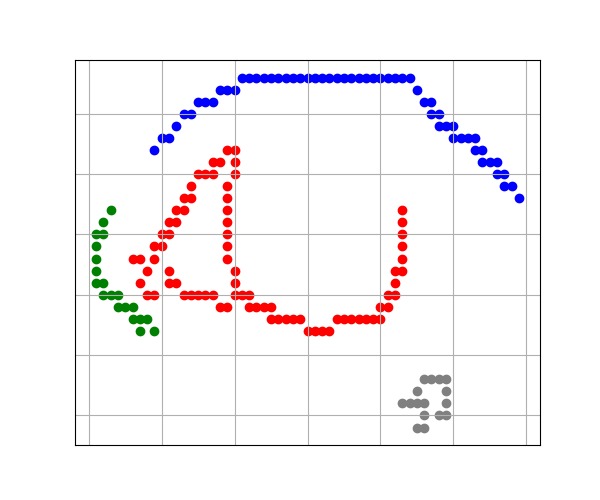
\includegraphics[width=0.9\linewidth]{fig/04_connected_components_right_eye.png}
        \legend{Maiores componentes conexos.}
        \label{fig:olho-grafo}
    \end{minipage}
    \hfill
    \begin{minipage}[b]{0.45\textwidth}
        \centering
        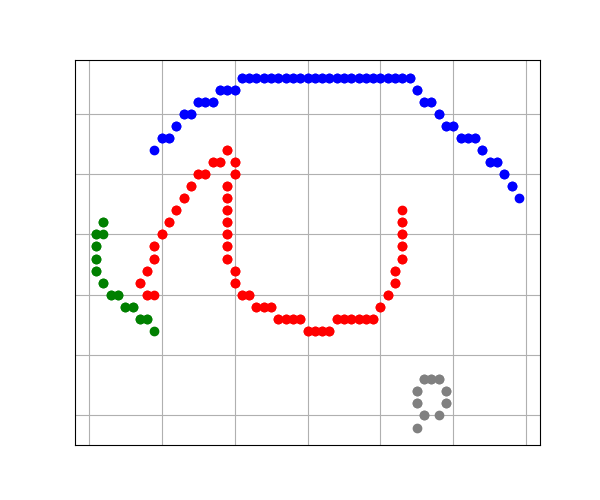
\includegraphics[width=0.9\linewidth]{fig/05_longest_path_right_eye.png}
        \legend{Aplicação da poda da AGM.}
        \label{fig:olho-agm}
    \end{minipage}

    \vspace{1cm}

    \begin{minipage}[b]{0.45\textwidth}
        \centering
        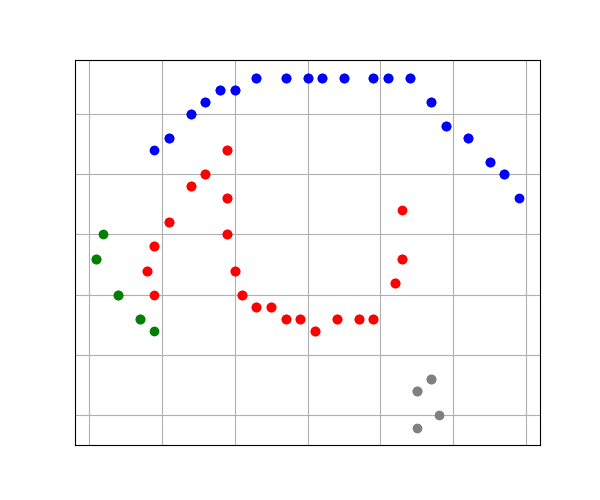
\includegraphics[width=1\linewidth]{fig/06_new_longest_path_right_eye.png}
        \legend{Remoção de alguns pontos de forma aleatória.}
        \label{fig:olho-aleatorio}
    \end{minipage}
    \label{fig:resultado-agm}
\end{figure}
\chapter{\textit{SPLINES} CÚBICAS} \label{cha:splines}

As \textit{splines} são funções definidas por partes que permitem a construção de curvas suaves a partir de um conjunto de pontos de controle. Elas são amplamente utilizadas em contextos onde é necessário representar formas complexas de maneira precisa e contínua, como na computação gráfica, modelagem geométrica e análise de dados. Dentre os diversos tipos, as \textit{splines} cúbicas se destacam por proporcionarem um bom equilíbrio entre flexibilidade e suavidade, garantindo continuidade até a segunda derivada e, consequentemente, uma transição harmoniosa entre os segmentos da curva.

Na área de biometria facial, a representação precisa das características do rosto -- como contornos dos olhos, nariz e lábios -- é essencial para o desempenho de sistemas de reconhecimento. Utilizar \textit{splines} para descrever essas formas permite capturar variações sutis da geometria facial com suavidade e fidelidade, o que é especialmente importante na comparação entre diferentes imagens. Além disso, a estrutura matemática das \textit{splines} facilita tanto a manipulação quanto a análise das curvas faciais, tornando-as uma ferramenta eficiente e robusta nesse tipo de aplicação.

Neste capítulo, serão abordadas as \textit{splines} cúbicas, suas propriedades e aplicações. A sua construção envolve a definição de um conjunto de pontos de controle e a determinação dos coeficientes que definem os polinômios cúbicos entre esses pontos. A suavidade da curva é garantida pela imposição de condições de continuidade e diferenciabilidade, resultando em uma representação suave e flexível.

\section{Definição de \textit{Splines} Cúbicas}
\label{sec:definicao-splines-cubicas}
Uma \textit{spline} cúbica é uma função definida por partes, onde cada parte é um polinômio cúbico. Dão-se, então, os polinômios de grau 3, que são especificados na forma canônica
\begin{equation}
    \vetor{p}(t) = \vetor{c_0} + \vetor{c_1}t + \vetor{c_2}t^2 + \vetor{c_3}t^3,
\end{equation}
onde $t$ é o parâmetro de interpolação e cada $\vetor{c_i}$ é um vetor no $\mathbb{R}^2$. A função $\vetor{p}(t)$ representa uma curva parametrizada com variável independente \( t \in [0,1] \). Essa função descreve a posição ao longo da curva no plano bidimensional, sendo essa posição o elemento de interesse ao desenharmos a curva, já que o processo de plotagem envolve a determinação de pontos com coordenadas $(x, y)$. Em outras palavras, as splines cúbicas são definidas por equações paramétricas, ou seja, ambas as componentes $x$ e $y$ são expressas como funções da variável $t$.

As curvas de Hermite são uma forma alternativa de representar curvas cúbicas. Expressar uma curva cúbica na forma de Hermite consiste em fornecer quatro valores fundamentais -- conhecidos como valores de Hermite -- que contêm todas as informações necessárias para descrever completamente a curva. Esses valores também permitem calcular os coeficientes da variável \( t \) na equação polinomial cúbica padrão, resultando assim na expressão completa da curva como um polinômio.

A principal motivação para utilizar a forma de Hermite está na possibilidade de determinar os coeficientes do polinômio diretamente a partir de informações conhecidas: a posição do ponto inicial da curva, \( \vetor{p_0} = \vetor{p}(0) \); a posição do ponto final, \( \vetor{p_1} = \vetor{p}(1) \); além das tangentes nesses pontos, ou seja, a taxa de variação da curva em \( \vetor{p_0} \), denotada por \( \vetor{v_0} = \vetor{v}(0) \), e em \( \vetor{p_1} \), denotada por \( \vetor{v_1} = \vetor{v}(1) \).


Agora que se conhecem os valores de Hermite, é possível resolvê-los através do sistema de equações
\begin{align}
    \vetor{p}(0) &= \vetor{c_0} + \vetor{c_1}(0) + \vetor{c_2}(0)^2 + \vetor{c_3}(0)^3 = \vetor{c_0}, \\
    \vetor{p}(1) &= \vetor{c_0} + \vetor{c_1} + \vetor{c_2} + \vetor{c_3}.
\end{align}
Para encontrar $v_0$ e $v_1$ é necessário calcular a derivada da posição. Portanto
\begin{align}
    \vetor{v}(t) &= \dfrac{d}{dt}\vetor{p}(t) = \vetor{c_1} + 2\vetor{c_2}t + 3\vetor{c_3}t^2,\\
    \vetor{v}(0) &= \vetor{c_1},\\
    \vetor{v}(1) &= \vetor{c_1} + 2\vetor{c_2} + 3\vetor{c_3}.
\end{align}
Então é possível obter a fórmula
\begin{align}
    \vetor{c_0} &= \vetor{p_0},\\
    \vetor{c_1} &= \vetor{v_0},\\
    \vetor{c_2} &= -3\vetor{p_0} - 2\vetor{v_0} - \vetor{v_1} + 3\vetor{p_1},\\
    \vetor{c_3} &= 2\vetor{p_0} + \vetor{v_0} + \vetor{v_1} - 2\vetor{p_1}. 
\end{align}
Escrevendo na forma matricial de Hermite, é obtida a expressão
\begin{equation}
    \vetor{p}(t) =  
        \left(
        \begin{array}{rrrr}
            1 & t & t^2 & t^3
        \end{array}\right)
        \left(
        \begin{array}{rrrr}
            1 & 0 & 0 & 0 \\
            0 & 0 & 1 & 0 \\
            -3 & 3 & -2 & -1 \\
                2 & -2 & 1 & 1
        \end{array}\right)
    \left(
        \begin{array}{r}
            \vetor{p_0} \\
            \vetor{p_1} \\
            \vetor{v_0} \\
            \vetor{v_1}
        \end{array}\right).
 \end{equation}

 \subsection{Criação da \textit{Spline}}

 Supondo que existam 4 pontos e é desejado criar uma \textit{spline} que passe por todos eles, é necessário criar 3 segmentos de curvas cúbicas, cada uma passando por dois pontos consecutivos. Assim, a \textit{spline} será composta por 3 segmentos cúbicos, cada um definido por 4 pontos de controle \cite{CatmullRom}.

 A primeira curva irá de $\vetor{p_0}$ a $\vetor{p_1}$, a segunda de $\vetor{p_1}$ a $\vetor{p_2}$ e a final de $\vetor{p_2}$ a $\vetor{p_3}$. Então é aplicada a fórmula que foi derivada acima para $\vetor{p_t}$, mas em 3 variantes diferentes, cada variante com um par diferente de pontos iniciais e finais. A fórmula da primeira curva terá pontos iniciais e finais $\vetor{p_0}$ e $\vetor{p_1}$, a segunda em $\vetor{p_1}$ e $\vetor{p_2}$ e a terceira em $\vetor{p_2}$ e $\vetor{p_3}$, como é possível ver na \autoref{fig:spline_tangentes}. No que diz respeito às tangentes, \citet{CatmullRom} propuseram uma abordagem baseada na diferença entre pontos adjacentes: a tangente em um ponto pode ser obtida subtraindo-se o ponto anterior do ponto seguinte. Por exemplo, a tangente no ponto $\vetor{p_2}$ é dada por $\vetor{p_3} - \vetor{p_1}$. É comum, ainda, dividir esse resultado por 2, pois essa operação tende a produzir curvas visualmente mais suaves e esteticamente agradáveis. Logo, é possível reescrever a equação em termos de quatro pontos ($\vetor{p_0}$ a $\vetor{p_3}$).


\begin{figure}[h!]
    \caption{CURVAS CÚBICAS DE CATMULL-ROM.}
    \centering
    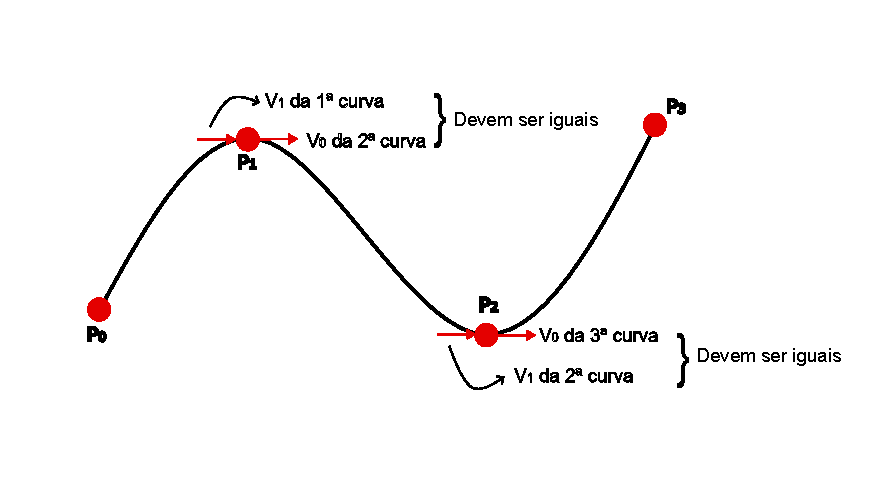
\includegraphics[width=0.8\textwidth]{fig/sp1.pdf}
    \legend{\textit{Spline} cúbica com 4 pontos de controle}
    \vspace{0.5em} % Espaçamento vertical entre as imagens
    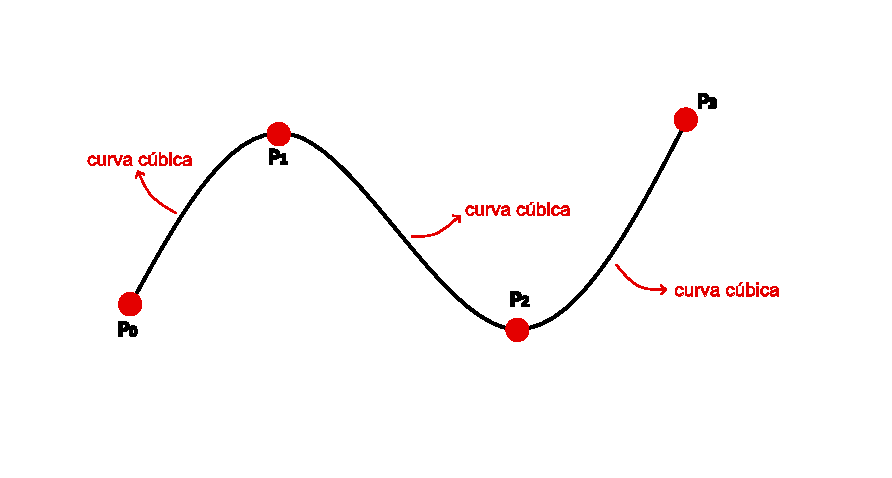
\includegraphics[width=0.8\textwidth]{fig/sp2.pdf}
    \legend{Tangentes coincidentes nas conexões das cúbicas em cada ponto.}
    \legend{FONTE: A autora.}
    \label{fig:spline_tangentes}
\end{figure}


Outra complicação que surge é que, ao se utilizar o ponto anterior e o ponto seguinte para o cálculo das tangentes, surge a dúvida sobre qual deve ser considerado o ponto anterior ao ponto inicial, $\vetor{p_i}$, e o ponto seguinte ao ponto final, $\vetor{p_f}$. Uma solução comum para esse problema é a adição de \textit{pontos fantasmas}, que não fazem parte da curva, mas são utilizados apenas para o cálculo das tangentes.


Então ficamos com
\begin{equation}
    \vetor{p}(t) =  
        \left(
        \begin{array}{rrrr}
            1 & t & t^2 & t^3
        \end{array}
        \right)
        \left(
        \begin{array}{rrrr}
            1 & 0 & 0 & 0 \\
            0 & 0 & 1 & 0 \\
            -3 & 3 & -2 & -1 \\
                2 & -2 & 1 & 1
        \end{array}
        \right)
    \left(
        \begin{array}{r}
            \vetor{p_1} \\
            \vetor{p_2} \\
            \frac{\vetor{p_2} - \vetor{p_0}}{2\tau} \\
                \frac{\vetor{p_3} - \vetor{p_1}}{2\tau}
        \end{array}
        \right),
\end{equation}
onde $\tau$ é um fator de escala que pode ser ajustado para controlar a suavidade da curva. O valor de $\tau$ pode ser definido com base na distância entre os pontos de controle ou em outras considerações geométricas. Com isso é possível chegar no formato de Catmull-Rom
\begin{equation}
    \vetor{p}(t) = \frac{1}{2}
       \left(
 	\begin{array}{rrrr}
 		1 & t & t^2 & t^3
 	\end{array}
    \right)
    \left(
 	\begin{array}{rrrr}
 		0 & 2 & 0 & 0 \\
 	    -\tau & 0 & \tau & 0 \\
 		2\tau & \tau-6 & -2(\tau-3) & -\tau \\
            -\tau & 4-\tau & \tau-4 & \tau
 	\end{array}
    \right)
   \left(
 	\begin{array}{r}
 		\vetor{p_0} \\
 	    \vetor{p_1} \\
 		\vetor{p_2} \\
            \vetor{p_3}
 	\end{array}
    \right).
\end{equation}

Na \autoref{fig:tensao} é possível observar que quanto menor a tensão $\tau$, menos suave fica a curva.

\begin{figure}[h!]
    \caption{TENSÃO DA CURVA.}
    \centering
    \begin{minipage}[b]{0.45\textwidth}
        \centering
        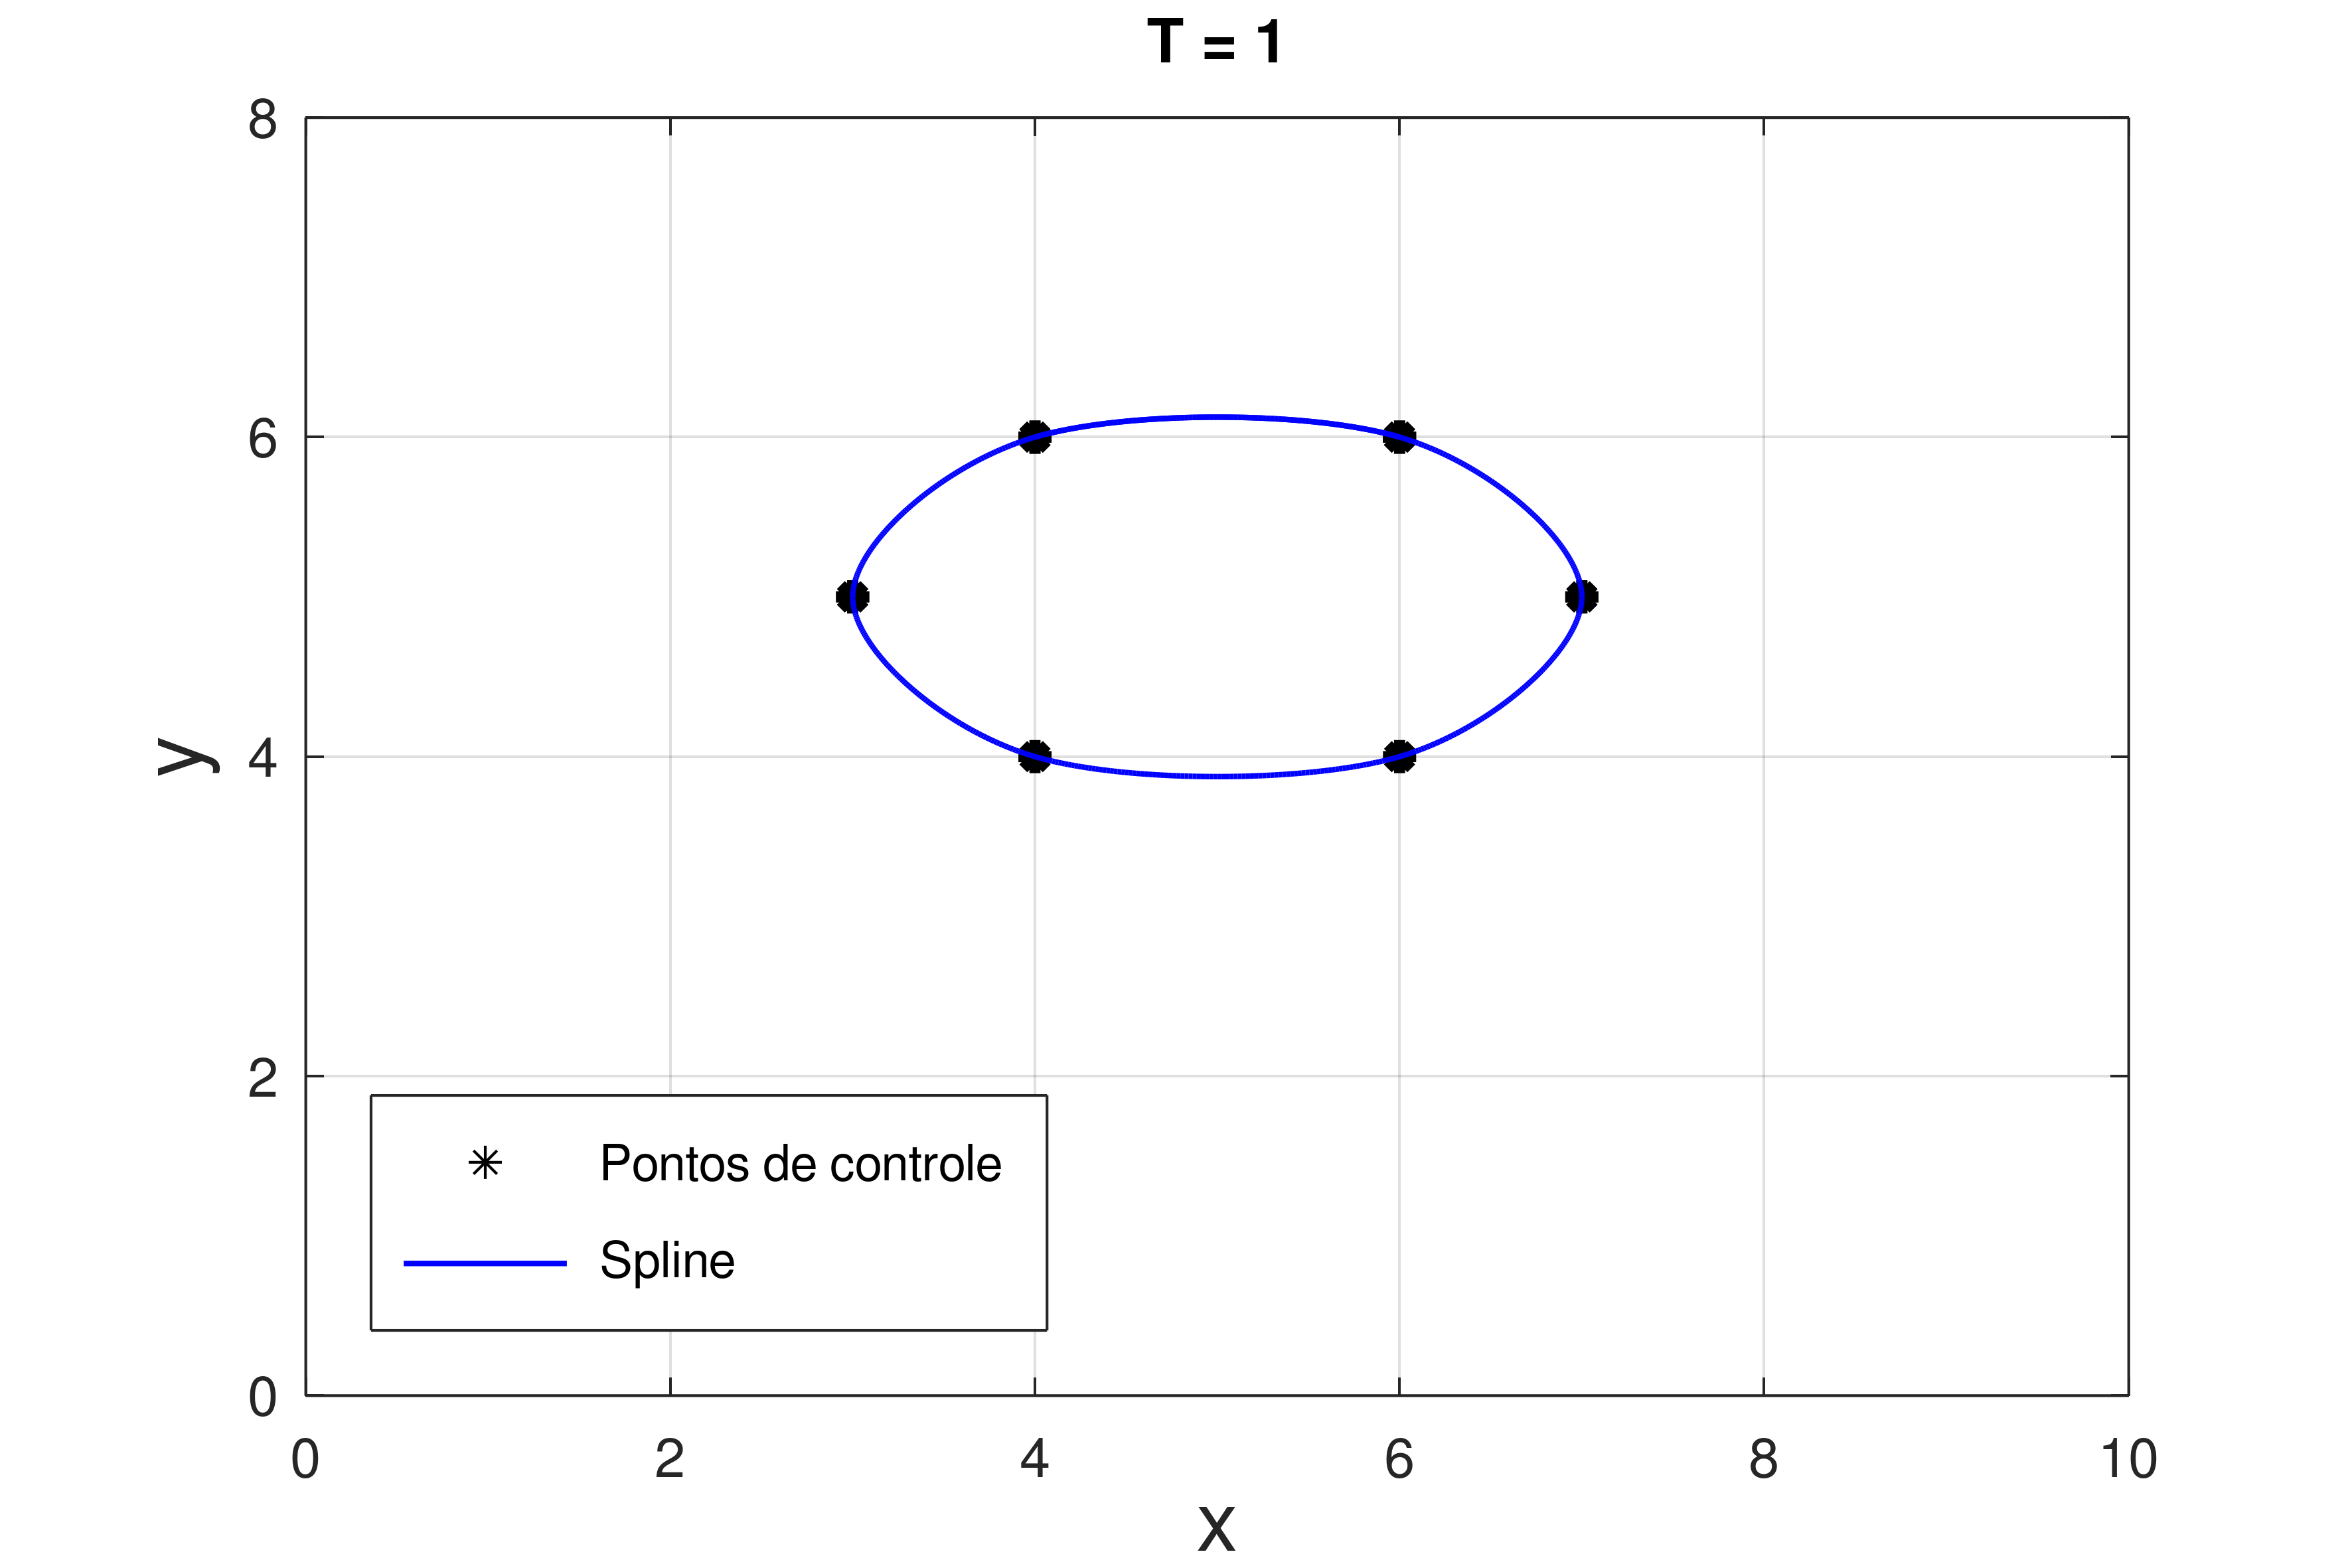
\includegraphics[width=1\linewidth]{fig/cat_rom_t1.png}
        \legend{$\tau$ = 1.}
        \label{fig:tesao1}
    \end{minipage}
    \hfill
    \begin{minipage}[b]{0.45\textwidth}
        \centering
        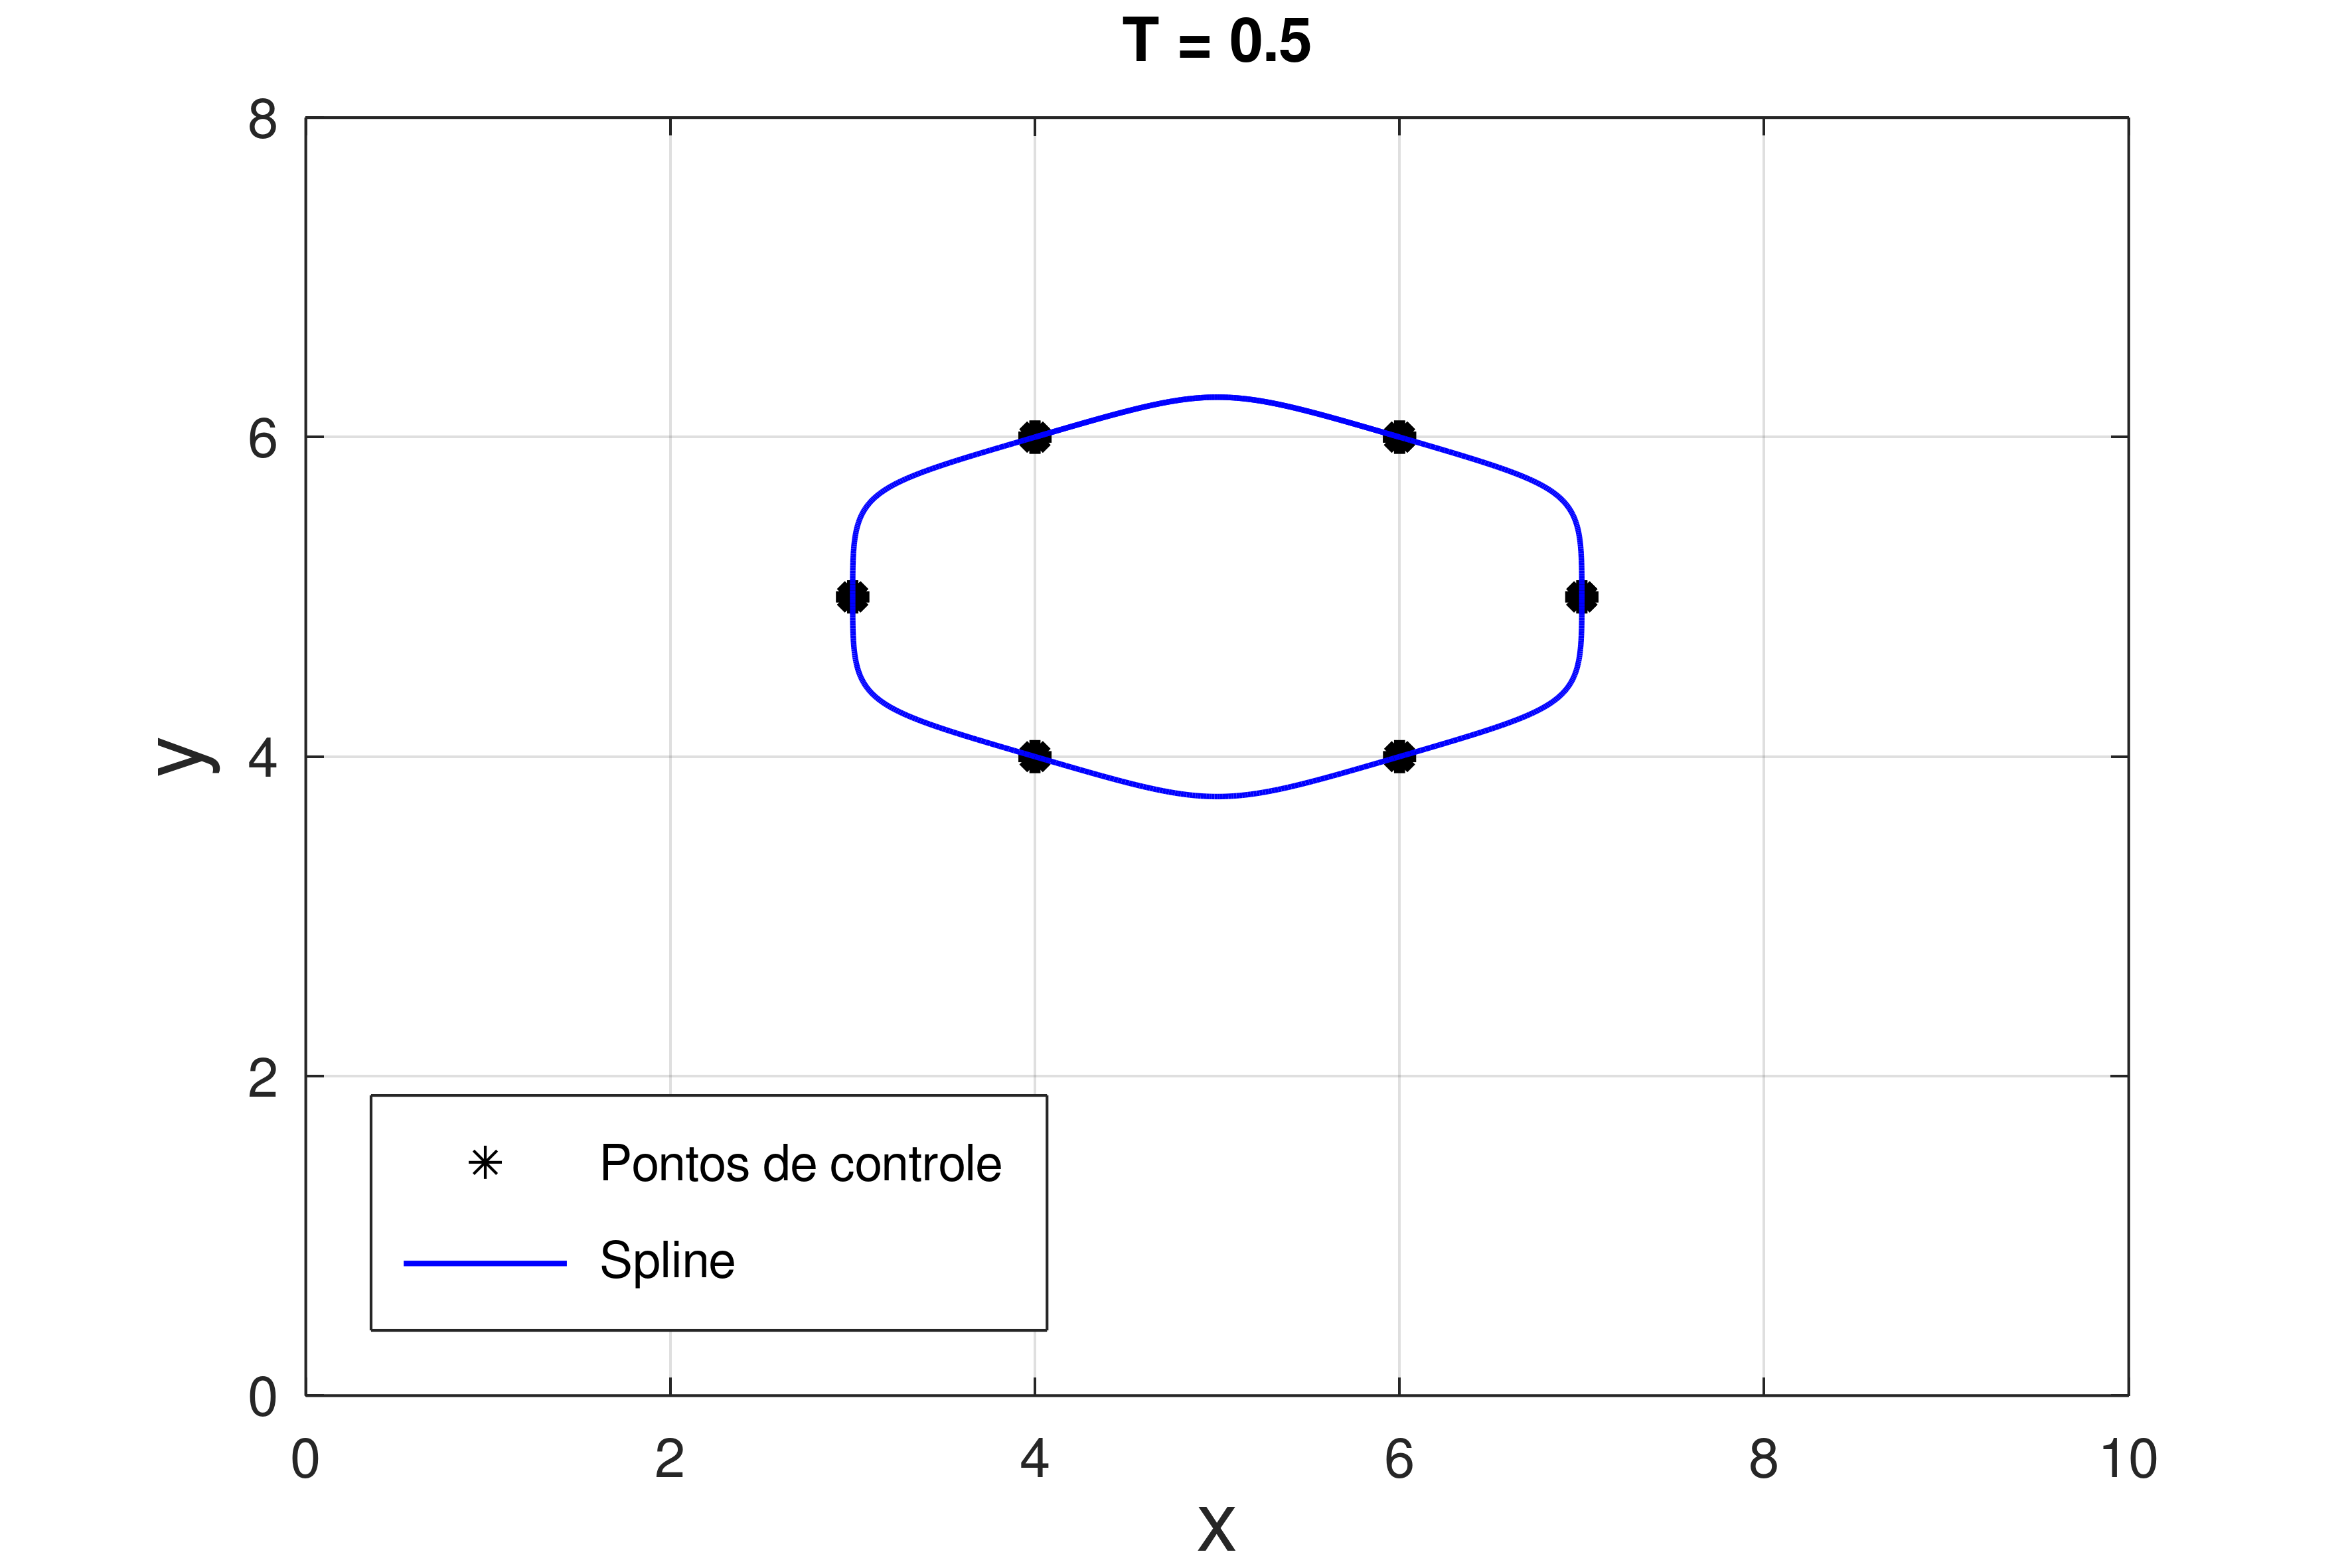
\includegraphics[width=1\linewidth]{fig/cat_rom_t05.png}
        \legend{$\tau$ = 0.5.}
        \label{fig:tensao05}
    \end{minipage}

    \vspace{1cm}

    \begin{minipage}[b]{0.45\textwidth}
        \centering
        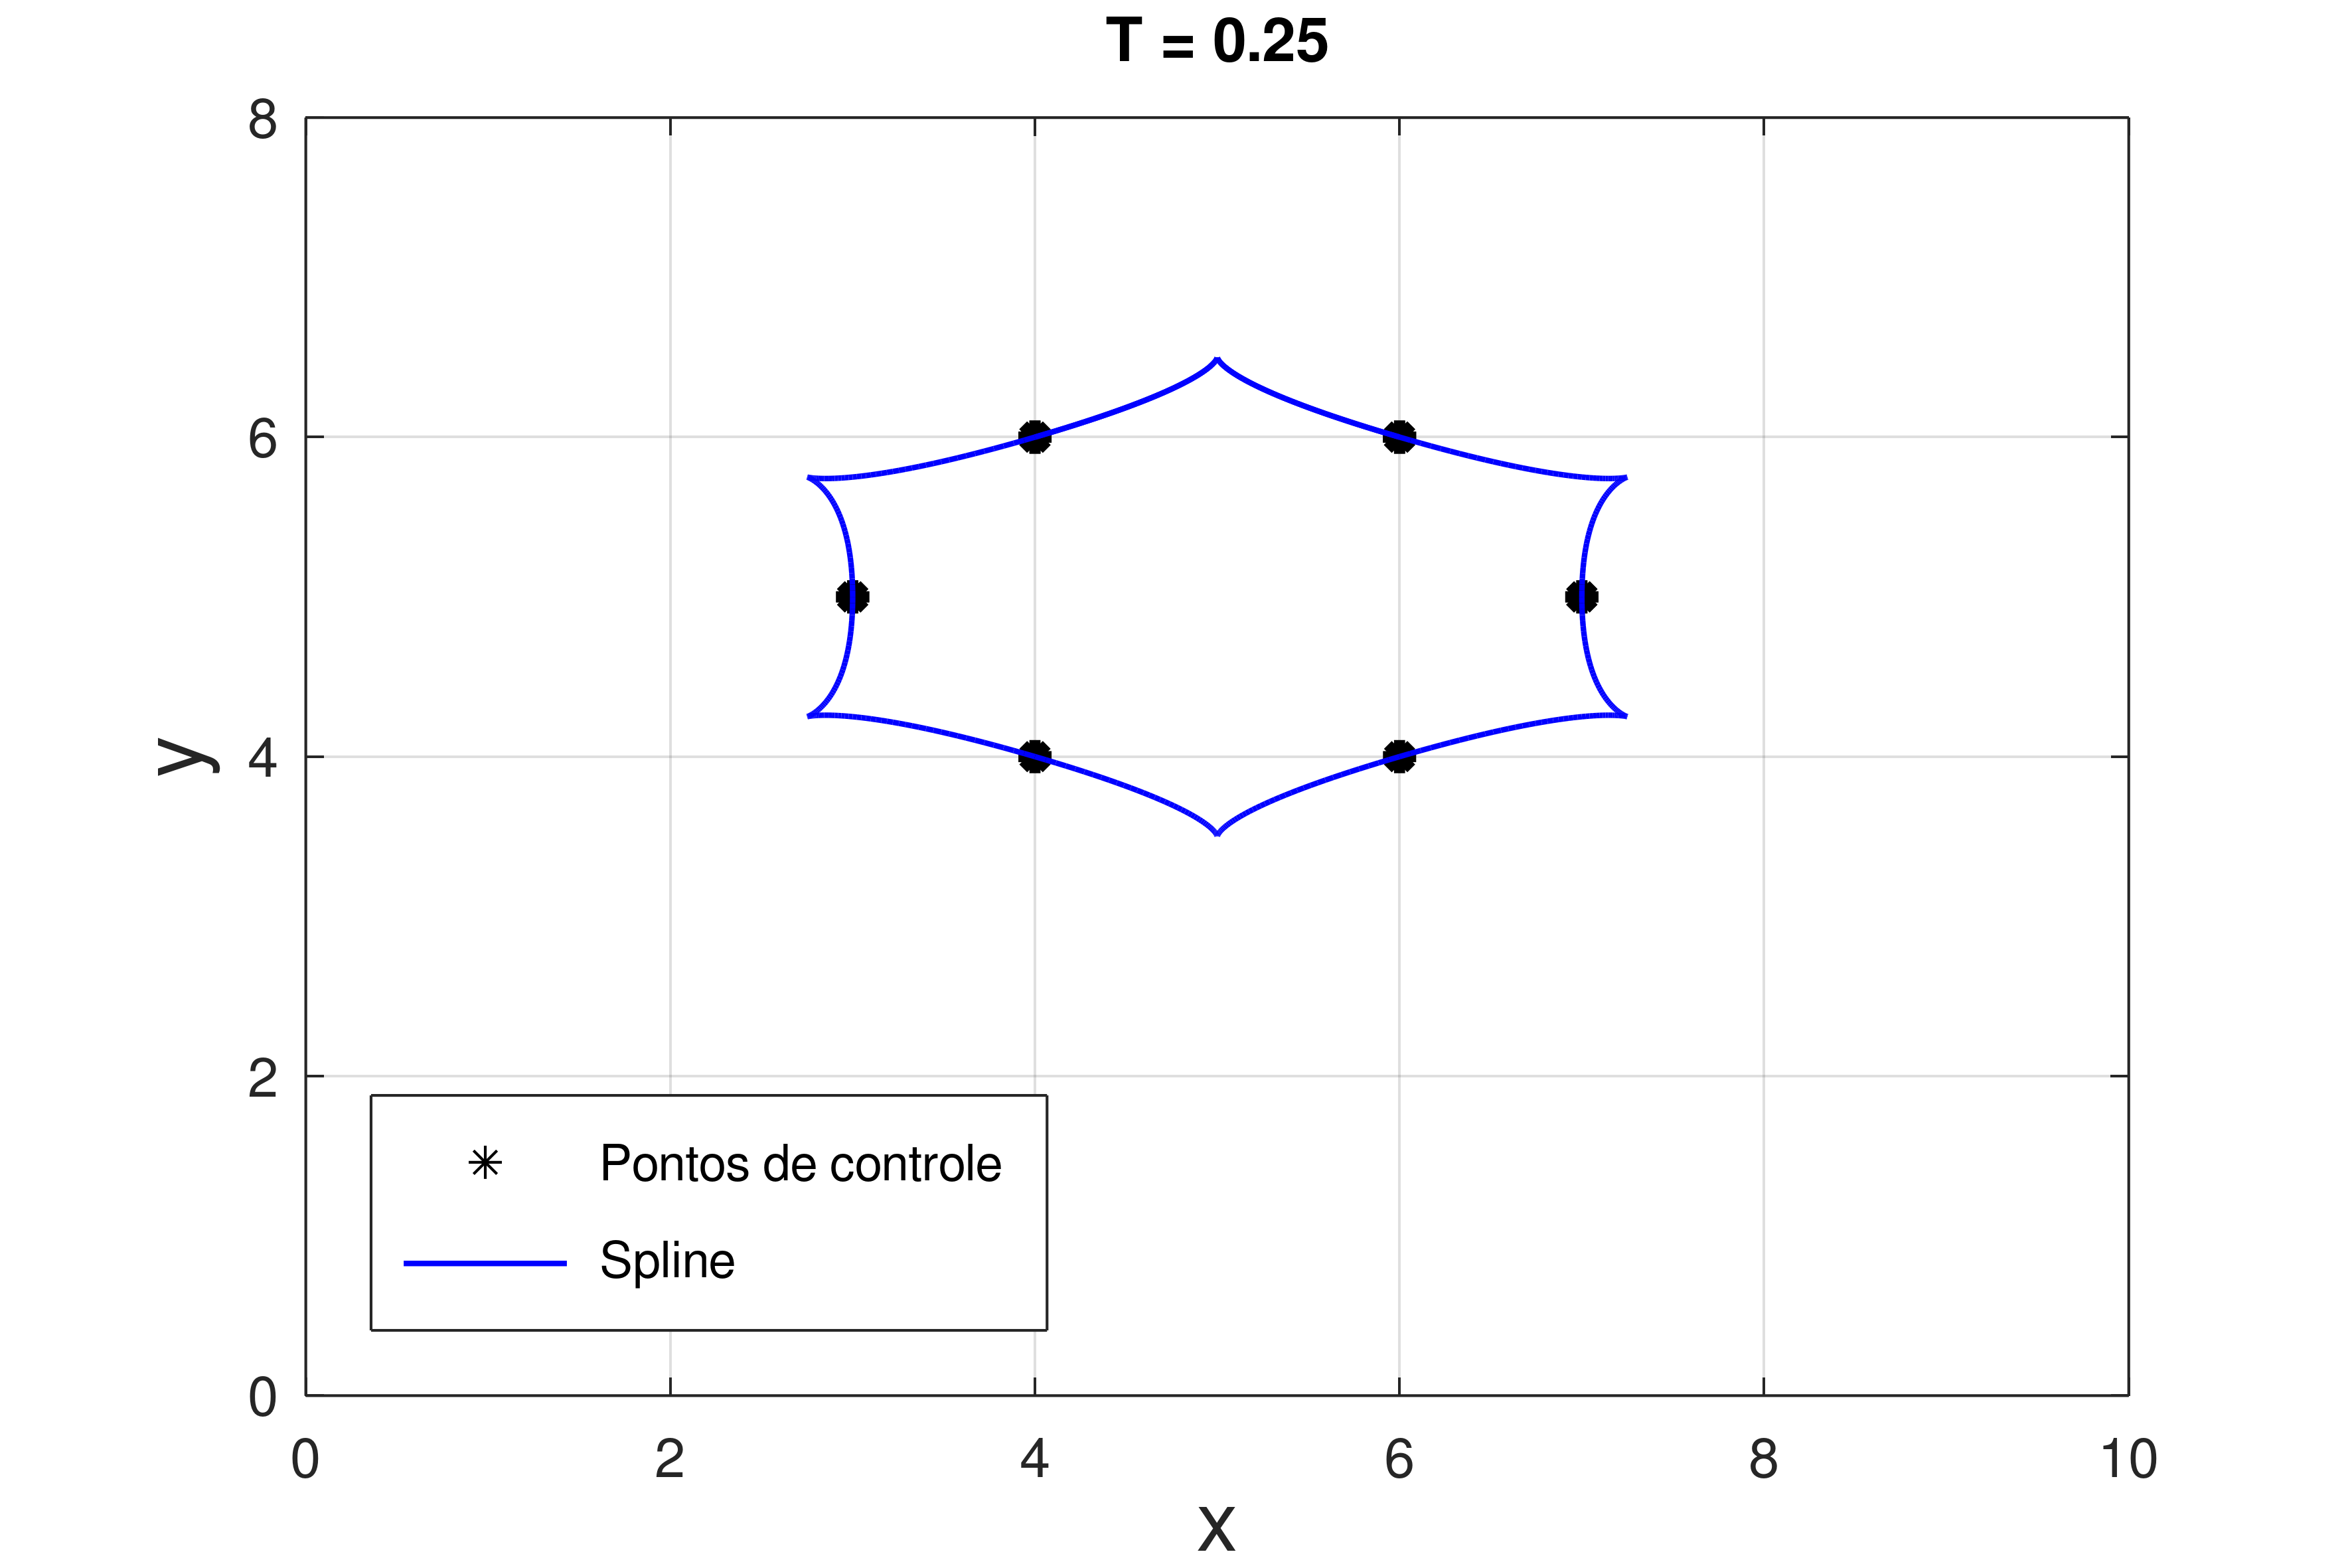
\includegraphics[width=1\linewidth]{fig/cat_rom_t025.png}
        \legend{$\tau$ = 0.25.}
        \label{fig:tensao025}
    \end{minipage}
    \label{fig:tensao}
    \legend{FONTE: A autora.}
\end{figure}

\subsection{Resultados}

Foi implementado um algoritmo autoral que gera uma \textit{spline} cúbica a partir de um conjunto de pontos de controle. O algoritmo proposto utiliza a fórmula de Catmull-Rom para calcular os coeficientes da curva, garantindo suavidade e continuidade. 

A \autoref{fig:splines_resultados} apresenta os resultados obtidos a partir de conjuntos de pontos de controle extraídos da imagem, conforme o processo descrito no \autoref{cha:processamento-imagem}. É importante ressaltar que os pontos foram reordenados de modo a garantir que a curva resultante seja traçada sempre da esquerda para a direita, o que é essencial para o bom desempenho do algoritmo de DTW.


\begin{figure}[h!]
    \caption{\textit{SPLINES} NOS PONTOS EXTRAÍDOS.}
    \centering
    \begin{minipage}[b]{0.45\textwidth}
        \centering
        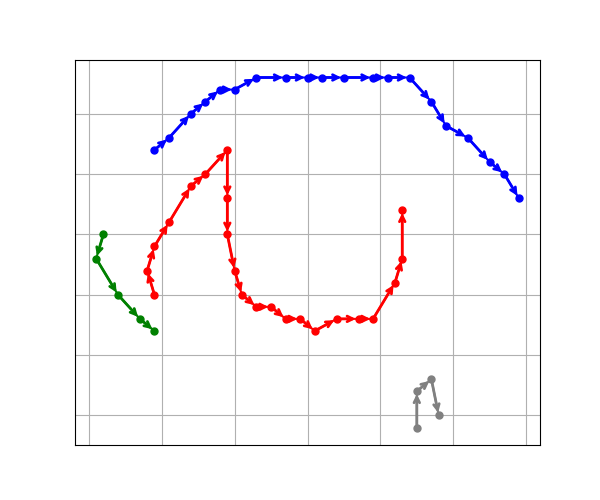
\includegraphics[width=1\linewidth]{fig/07_sorted_points_right_eye.png}
        \legend{Reordenação dos pontos.}
        \label{fig:reordenacao}
    \end{minipage}
    \hfill
    \begin{minipage}[b]{0.45\textwidth}
        \centering
        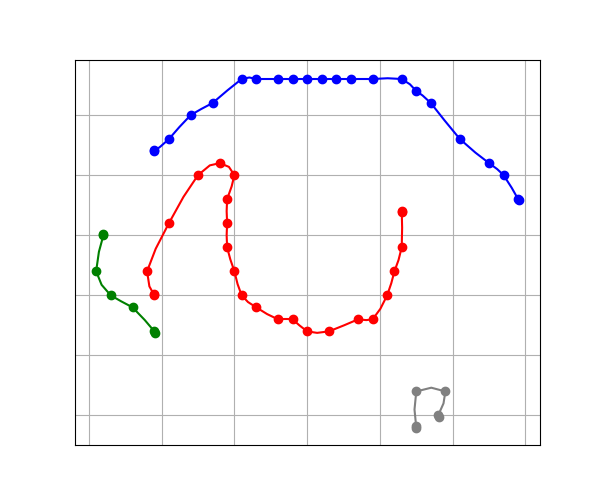
\includegraphics[width=1\linewidth]{fig/08_spline_plot_right_eye.png}
        \legend{\textit{Splines}.}
        \label{fig:spline}
    \end{minipage}
    \label{fig:splines_resultados}
    \legend{FONTE: A autora.}
\end{figure}





% \begin{algorithm}[H]
%     \renewcommand{\algorithmcfname}{Algoritmo}%
%     \SetAlgoLined
%     \eSe{$n\leq r$}{
%         Calcule a fatoração $\vetor{M}=\vetor{LU}$ por outro método\;
%     }{
%         Calcule a fatoração $\left[\begin{array}{cc} \vetor{A}\\\vetor{C}\end{array}\right]=\left[\begin{array}{cc} \vetor{L_{11}}\\\vetor{L_{21}}\end{array}\right]\vetor{U_{11}}$\;
%         Calcule $\vetor{U_{12}}=\vetor{L_{11}^{-1}}\vetor{B}$ pela solução do sistema linear $\vetor{L_{11}}\vetor{U_{12}}=\vetor{B}$\;
%         $\vetor{\tilde{D}} \gets \vetor{D}-\vetor{L_{21}}\vetor{U_{12}}$\;
%         Calcule a fatoração $\vetor{\tilde{D}}=\vetor{L_{22}}\vetor{U_{22}}$ recursivamente\;
%         Retorne $\vetor{L}=\left[\begin{array}{cc} \vetor{L_{11}} & \vetor{0}\\\vetor{L_{21}} & \vetor{L_{22}}\end{array}\right]$ e $\vetor{U}=\left[\begin{array}{cc} \vetor{U_{11}} & \vetor{U_{12}}\\\vetor{0} & \vetor{U_{22}}\end{array}\right]$\;
%     }
% \end{algorithm}

% \begin{algorithm}
%     \caption{Fatoração QR magra de uma matriz $\vetor{A}\in\R^{m\times n}$ usando Gram-Schmidt.}
%     \SetAlgoLined
%     \Para{$k$ de $1$ até $n$}{
%         $\vetor{v_k} \gets \vetor{A}[:,k]$\;
%         \Para{$i$ de $1$ até $k-1$}{
%             $\vetor{R}[i,k] \gets \vetor{Q}[:,i]^{\vetor{T}}\vetor{A}[:,k]$\;
%             $\vetor{v_k} \gets \vetor{v_k}-\vetor{R}[i,k]\vetor{Q}[:,i]$\;
%         }
%         $\vetor{R}[k,k]\gets\left\|\vetor{v_k}\right\|_2$\;
%         $\vetor{Q}[:,k]\gets\dfrac{1}{\vetor{R}[k,k]}\vetor{v_k}$\;
%     }
%     \label{alg:QRmagra}
% \end{algorithm}
\chapter{\textit{DYNAMIC TIME WARPING}} \label{cha:dtw}

O \textit{Dynamic Time Warping} (DTW) \cite{tavenard.blog.dtw} é um algoritmo amplamente utilizado para medir a similaridade entre duas sequências temporais que podem variar em velocidade, tempo ou comprimento. Sua principal aplicação está em áreas como reconhecimento de fala, análise de séries temporais, bioinformática e visão computacional. Neste trabalho, essa técnica é utilizada para comparação entre as curvas que representam as características faciais dos indivíduos, permitindo identificar as mesmas pessoas em diferentes momentos ou condições.

\section{Introdução}

Este algoritmo surgiu como uma solução para o problema de comparação entre sequências temporais que apresentam distorções no eixo do tempo. Diferente da distância Euclidiana, que compara ponto a ponto, o DTW permite alinhar dinamicamente duas sequências, encontrando o menor custo de distorção temporal necessário para que elas se assemelhem.

Considere duas sequências temporais
\begin{equation}
    X = (x_1, x_2, \ldots, x_n) \quad \text{e} \quad Y = (y_1, y_2, \ldots, y_m),
\end{equation}
onde \(X\) e \(Y\) são as sequências a serem comparadas, com \(n\) e \(m\) sendo seus respectivos comprimentos.

O algoritmo de DTW constrói uma matriz de custo acumulado \(D\) de dimensão \(n \times m\), na qual cada elemento \(D(i, j)\) representa o custo mínimo acumulado para alinhar os primeiros \(i\) elementos de \(X\) com os primeiros \(j\) elementos de \(Y\).

O alinhamento entre os primeiros elementos das sequências ocorre diretamente na célula \(D(1,1)\), definida
\begin{equation}
    D(1,1) = d(x_1, y_1),
\end{equation}
onde \(d(x_1, y_1)\) é a distância entre os primeiros elementos de cada sequência, usualmente calculada por uma métrica como a distância Euclidiana.

Em seguida, são preenchidas a primeira linha e a primeira coluna da matriz. Nessas bordas, o caminho de alinhamento é único (ou apenas vertical ou apenas horizontal), o que resulta em uma soma cumulativa de distâncias. 
\begin{align}
    D(i,1) &= d(x_i, y_1) + D(i-1,1), \quad \text{para } i = 2, \ldots, n, \\
    D(1,j) &= d(x_1, y_j) + D(1,j-1), \quad \text{para } j = 2, \ldots, m.
\end{align}

Essa etapa garante que todas as possíveis trajetórias de alinhamento que passam pelas extremidades da matriz possam ser consideradas no cálculo recursivo subsequente.

\subsubsection*{Preenchimento recursivo da matriz}

A partir de \(i = 2\) e \(j = 2\), a matriz é preenchida utilizando a fórmula recursiva do DTW
\begin{equation}
    D(i, j) = d(x_i, y_j) + \min \begin{cases}
        D(i-1, j), \\
        D(i, j-1), \\
        D(i-1, j-1),
    \end{cases}
    \quad \text{para } i \geq 2 \text{ e } j \geq 2.
\end{equation}

Essa relação computa o custo acumulado de alinhar \(x_i\) com \(y_j\). O valor final \(D(n, m)\) representa o custo total do alinhamento ótimo entre as duas sequências temporais.


A \autoref{fig:dtw_intro} ilustra o conceito de alinhamento dinâmico, mostrando como o DTW pode distorcer o eixo do tempo para alinhar duas sequências temporais que, à primeira vista, parecem diferentes.

\begin{figure}[h!]
    \centering
    \caption{ALINHAMENTO DINÂMICO.}
    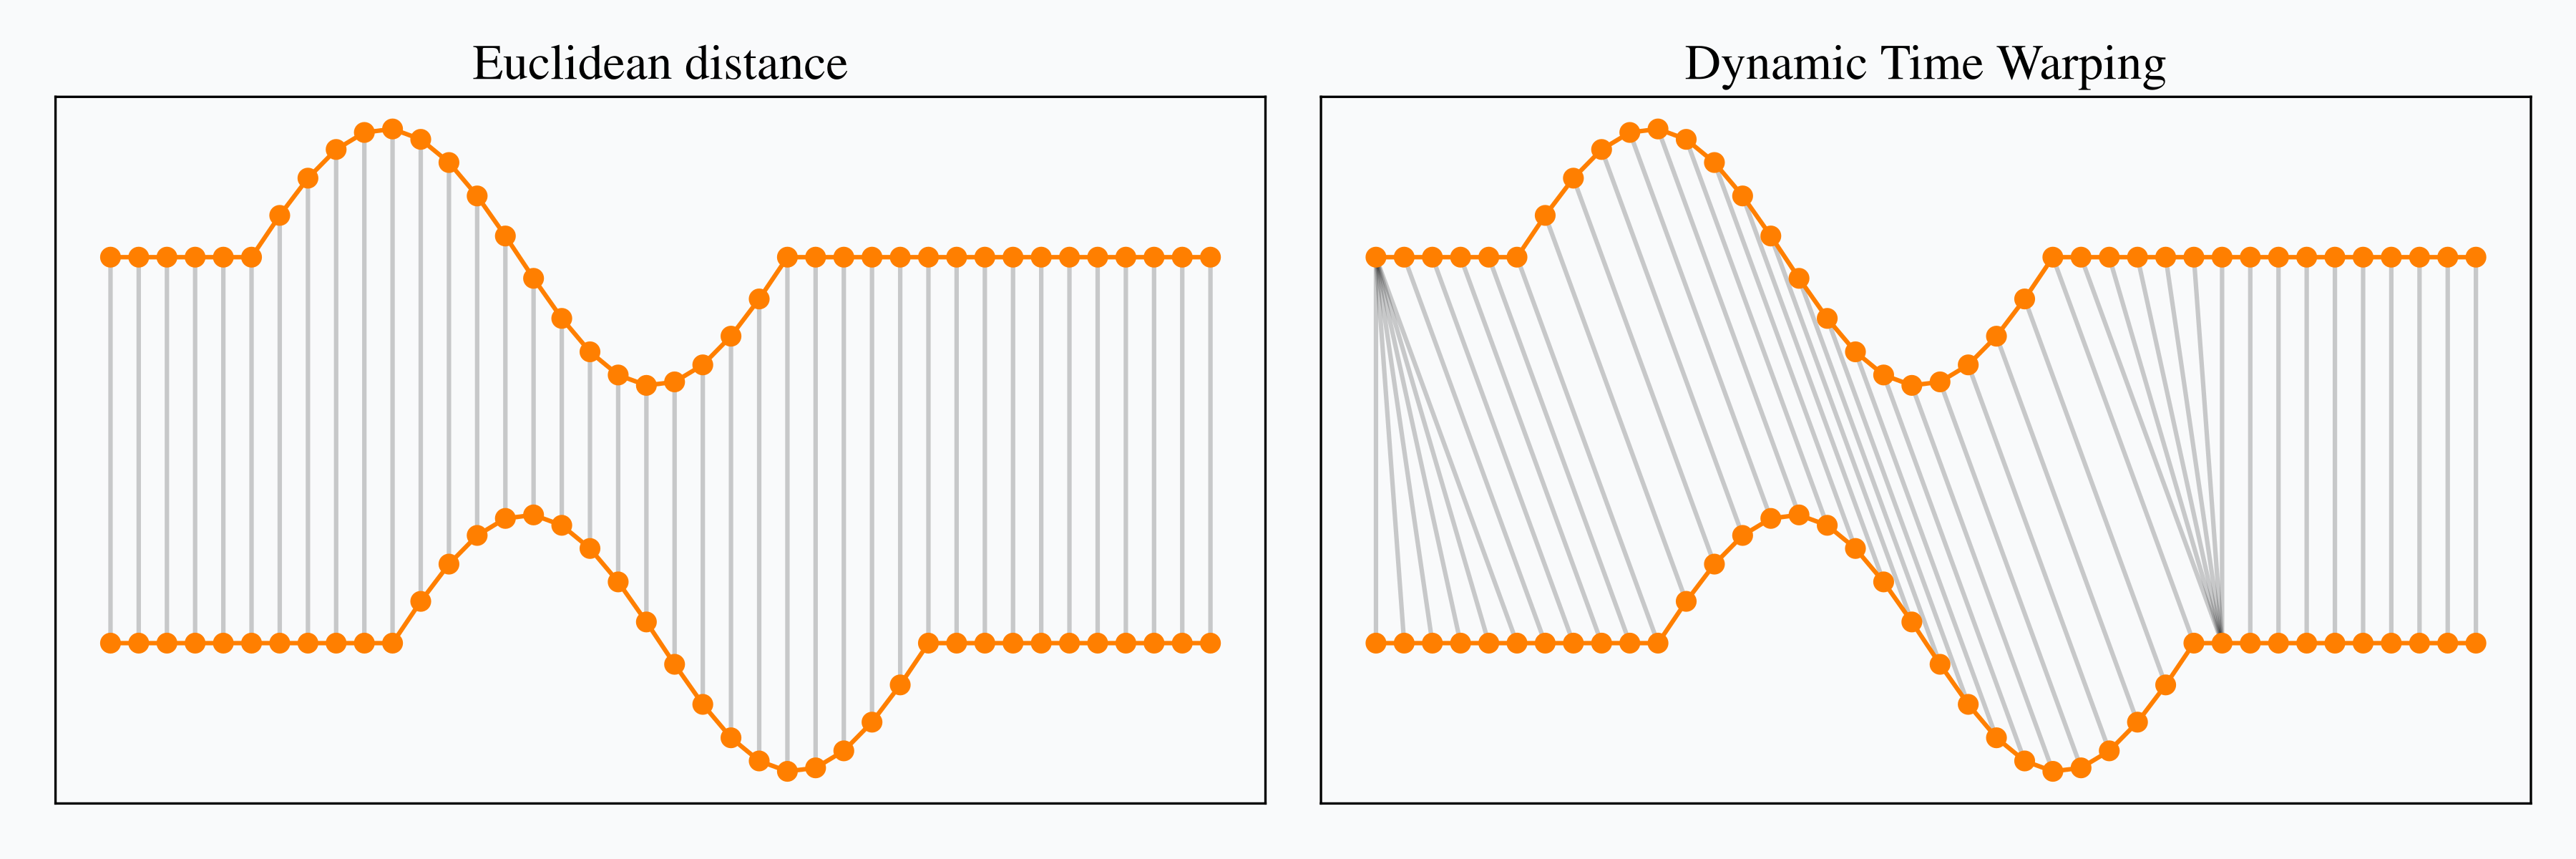
\includegraphics[width=0.8\textwidth]{fig/dtw_vs_euc.png}
    \legend{FONTE: \cite{tavenard.blog.dtw}}
    \label{fig:dtw_intro}
\end{figure}

\section{Vantagens e Desvantagens}

O método apresenta diversas vantagens em relação a outras métricas de distância, como a distância Euclidiana. Entre elas, destacam-se:
\begin{itemize}
    \item \textbf{Robustez a variações de tempo}, permitindo lidar com sequências que apresentam diferenças de velocidade ou comprimento, o que possibilita comparações mais precisas.
    \item \textbf{Alinhamento dinâmico}, ao encontrar o melhor mapeamento entre as sequências, minimizando o custo total de distorção temporal.
    \item \textbf{Versatilidade}, com bom desempenho em sinais unidimensionais e multidimensionais, sendo aplicável em diversas áreas, como reconhecimento de padrões e análise de séries temporais.
\end{itemize}

No entanto, o DTW também possui desvantagens:
\begin{itemize}
    \item \textbf{Complexidade computacional} com \(O(n \cdot m)\), o que pode ser um limitante para sequências muito longas.
    \item \textbf{Sensibilidade a ruídos}, o que pode levar a alinhamentos incorretos.
\end{itemize}


\section{Justificativa para o seu uso}

Neste trabalho, o DTW foi utilizado por ser uma técnica adequada para comparar sequências que representam características espaciais extraídas de contornos faciais utilizando um algoritmo simples. As curvas resultantes dessas características podem variar em comprimento e forma devido a diferentes condições de iluminação, expressões faciais ou ângulos de captura. Esse método permite alinhar essas curvas de forma dinâmica, possibilitando uma comparação mais precisa entre elas.

Além disso, este trabalho baseia-se na abordagem proposta por \citet{DTW_LSTM}, que demonstraram a eficácia do uso do algoritmo DTW na comparação da variação das cores dos \textit{pixels} ao longo do vetor. Os autores obtiveram acurácias de 100\%, 94\% e 70\% em diferentes cenários experimentais, evidenciando a robustez do método. Observa-se, contudo, uma diminuição progressiva na acurácia à medida que ruídos são introduzidos nas imagens, o que reforça a importância de técnicas complementares de pré-processamento.


Entretanto, uma limitação relevante observada nesse estudo foi o alto custo computacional do DTW, o que compromete sua aplicabilidade em cenários que exigem processamento em tempo real. Embora o tempo exato de execução dos experimentos não tenha sido reportado pelos autores, implementamos um \textit{script} com base na proposta do artigo, cujo tempo de execução foi de aproximadamente 10 horas para comparar duas imagens representadas por vetores de dimensão 77.284 (correspondentes às intensidades de cinza). 

Foi utilizada a biblioteca \texttt{dtaidistance}  \cite{libDTW} para a implementação do DTW para reproduzir os resultados do artigo, pois os pixels das imagens são representados como vetores unidimensionais. Porém para o nosso trabalho foi preciso adaptar o código para lidar com coordenadas, o que exigiu uma abordagem diferente, visto que as curvas não são vetores unidimensionais, mas sim representações contínuas de pontos no espaço.


\chapter{RESULTADOS} \label{cha:resultados}

Para a avaliação dos métodos propostos neste trabalho, foi utilizada uma amostra do banco de dados FERET \cite{FERET1,FERET2}. A seleção compreende um total de 24 imagens faciais pertencentes a quatro indivíduos distintos. Ressalta-se que há um desbalanceamento na distribuição de imagens por indivíduo, sendo 10 imagens do primeiro sujeito, 3 do segundo, 6 do terceiro e 5 do quarto. Todas as imagens foram capturadas em condições controladas, com orientação frontal e sem variações significativas de ângulo ou expressões faciais.

Foram segmentadas quatro regiões distintas: olhos, nariz e boca. Cada uma é representada por um \textit{array} bidimensional que armazena as coordenadas dos pontos gerados pela aplicação das \textit{splines} em cada região.


O DTW foi aplicado separadamente para cada uma dessas quatro representações, permitindo avaliar a similaridade local (por região) e utilizando o sistema de votação para determinar a identidade do indivíduo. Além disso, uma outra versão com todas as características concatenadas foi utilizada como referência global da face.

É importante ressaltar que devido a uma aleatoriedade introduzida de propósito no algoritmo para retirar alguns pontos (\autoref{sec:resultado-agm}), os resultados podem variar entre as execuções. Portanto, para garantir a consistência dos resultados, foi utilizada a semente \texttt{random.seed(42)} em todas as execuções, assegurando que os mesmos pontos fossem selecionados em cada teste.

A máquina utilizada para os testes possui as seguintes especificações: processador Intel Core i7-8550U, 16 GB de memória RAM, 4 núcleos e 8 processadores lógicos.

\section{Parâmetros de Configuração}
\label{sec:parametros-configuracao}

Para a realização dos experimentos, foram definidos alguns parâmetros de configuração que influenciam diretamente o desempenho do DTW e a qualidade das curvas geradas pelas \textit{splines}. Esses parâmetros incluem:
\begin{itemize}
    \item \textbf{Passo da \textit{Spline}:} que define a densidade dos pontos ao longo da curva. Um passo menor resulta em curvas mais detalhadas, mas com maior custo computacional.
    \item \textbf{Tensão} que controla a suavidade das curvas geradas pelas \textit{splines}. Valores mais altos resultam em curvas mais flexíveis, enquanto valores mais baixos produzem curvas mais rígidas. %citar figura 11
    \item \textbf{Translação}, indicando se as curvas devem ser transladadas para alinhar melhor as características faciais.
\end{itemize}

Para cada combinação desses parâmetros, foram realizados testes com as características faciais concatenadas e segmentadas, permitindo uma análise comparativa dos resultados obtidos.

\section{Resultados Obtidos}

 As tabelas \ref{tab:resultados-concatenados} e \ref{tab:resultados-segmentados} apresentam os resultados obtidos para cada uma das abordagens, considerando diferentes parâmetros de configuração.

Esses resultados foram obtidos a partir do confronto individual entre as curvas geradas pelas splines das imagens faciais do banco de dados FERET. O processo consistiu em comparar a primeira imagem com as 23 restantes, a segunda com as 22 seguintes, e assim sucessivamente, até que todas as imagens fossem comparadas. A acurácia foi então calculada como a porcentagem de acertos em relação ao total de imagens.

\begin{table}[h!]
    \centering
    \caption{Testes realizados para as características concatenadas.}
    \begin{tabular}{|c|c|c|c|c|c|c|c|}
    \hline
    \textbf{Experimento} & \textbf{Passo \textit{Spline}} & \textbf{Tensão} & \textbf{Translação} & \textbf{Acurácia (\%)} & \textbf{Tempo} \\
    \hline
    1 & 0.5 & 1 & Não & 50 & 4min 21s\\
    2 & 0.5 & 0.5 & Não & 54.16 & 4min 05s\\
    3 & 0.5 & 0.25 & Não & 50 & 4min 13s\\

    4 & 1 & 1 & Não & 50 & 2min 02s\\
    5 & 1 & 0.5 & Não & 54.16 & 1min 48s\\
    6 & 1 & 0.25 & Não & 45.83 & 2min 00s\\

    7 & 0.5 & 1 & Sim & 16.66 & 4min 33s \\
    8 & 0.5 & 0.5 & Sim & 41.66 & 3min 57s \\
    9 & 0.5 & 0.25 & Sim & 37.5 & 5min 05s\\
 
    10 & 1 & 1 & Sim & 33.33 & 1min 58s \\
    11 & 1 & 0.5 & Sim & 33.33 & 2min 10s \\
    12 & 1 & 0.25 & Sim & 33.33 & 2min 04s \\
    \hline
    \end{tabular}
    \label{tab:resultados-concatenados}
\end{table}

\begin{table}[h!]
    \centering
    \caption{Testes realizados para as características segmentadas.}
    \begin{tabular}{|c|c|c|c|c|c|c|c|}
    \hline
    \textbf{Experimento} & \textbf{Passo \textit{Spline}} & \textbf{Tensão} & \textbf{Translação} & \textbf{Acurácia (\%)} & \textbf{Tempo} \\
    \hline

    13 & 0.5 & 1 & Não & 41.66 & 2min 12s \\
    14 & 0.5 & 0.5 & Não & 41.66 & 2min 39s \\
    15 & 0.5 & 0.25 & Não & 41.66 & 2min 21s \\
    
    16 & 1 & 1 & Não & 45.83 & 1min 07s \\
    17 & 1 & 0.5 & Não & 37.5 & 1min 08s \\
    18 & 1 & 0.25 & Não & 41.66 & 1min 08s \\
 
    19 & - & - & Não & 37.5 & 0min 21s\\
 
    20 & 0.5 & 1 & Sim & 79.16 & 2min 43s \\
    21 & 0.5 & 0.5 & Sim & 75 & 2min 39s \\
    22 & 0.5 & 0.25 & Sim & 70.83 & 2min 27s \\
 
    23 & 1 & 1 & Sim & 75 & 1min 04s \\
    24 & 1 & 0.5 & Sim & 79.16 & 1min 09s \\
    25 & 1 & 0.25 & Sim & 79.16 & 1min 13s \\
 
    26 & - & - & Sim & 70.83 & 0min 17s\\
    \hline
    \end{tabular}
    \label{tab:resultados-segmentados}
\end{table}

\subsection{Características Concatenadas}

Na Tabela \ref{tab:resultados-concatenados}, observa-se que a introdução de translação causou uma queda significativa na acurácia. Enquanto os experimentos sem translação atingiram até 54,16\% de acurácia (Experimentos 2 e 5), aqueles com translação tiveram desempenho inferior, com valores que variaram entre 16,66\% e 41,66\%. Isso sugere que, ao utilizar características concatenadas, a translação dificulta a extração de padrões discriminativos.

Além disso, ao comparar os valores de tensão, não há uma tendência clara de melhora ou piora na acurácia. No entanto, o passo da \textit{spline} igual a 1 reduziu consideravelmente o tempo de execução, com destaque para o Experimento 5 (1min 48s), mantendo a mesma acurácia de 54,16\% que o Experimento 2 (4min 05s), cujo passo era 0.5. Isso indica que um passo maior pode ser preferível por reduzir o tempo computacional sem comprometer o desempenho.

\subsection{Características Segmentadas}

Na Tabela \ref{tab:resultados-segmentados}, o cenário se inverte: os melhores resultados foram obtidos com a presença de translação. Os experimentos 20, 24 e 25 atingiram 79,16\% de acurácia, superando significativamente os demais. Isso indica que, no caso das características segmentadas, a translação introduz variações benéficas ao aprendizado, provavelmente por aumentar a robustez das representações faciais.

Entre os experimentos sem translação, a acurácia ficou abaixo de 46\%, indicando que a segmentação sozinha não é suficiente para gerar boas representações sem esse tipo de transformação. Já o tempo de execução foi consistentemente mais baixo nas segmentadas em comparação às concatenadas, sugerindo uma vantagem adicional em termos de eficiência computacional.

Os experimentos 19 e 26 utilizaram apenas os pontos extraídos automaticamente, sem aplicação de \textit{splines}. Esses testes funcionam como uma linha de base para comparação com as demais abordagens. Observa-se que, ao comparar o Experimento 19 com o Experimento 26, a acurácia salta de 37,5\% para 70,83\%, evidenciando o impacto positivo da translação mesmo quando se utiliza uma representação simples baseada apenas nos pontos faciais. Isso reforça a relevância da translação como uma etapa de pré-processamento importante, especialmente no contexto das características segmentadas.

\subsection{Considerações Finais}

De forma geral:
\begin{itemize}
    \item A translação impacta negativamente nas características concatenadas, mas melhora significativamente os resultados nas características segmentadas.
    \item Um passo da \textit{spline} maior (1) reduz o tempo computacional sem grandes perdas de desempenho.
    \item As características segmentadas com translação se mostraram a melhor combinação, atingindo a maior acurácia com tempos de execução relativamente baixos.
\end{itemize}

Esses resultados indicam que a segmentação, aliada a transformações geométricas simples como a translação, pode ser uma estratégia promissora para a extração de características mais robustas em sistemas biométricos baseados em curvas \textit{spline}.
\chapter{CONCLUSÃO} \label{cha:conclusao}

O objetivo central deste trabalho foi investigar a viabilidade do uso de \textit{splines} cúbicas como método de representação de características faciais em sistemas biométricos, buscando unir a expressividade matemática das curvas suaves com a necessidade de precisão e eficiência nos processos de identificação de indivíduos. Diferentemente de abordagens tradicionais baseadas em pixels, esta proposta parte da premissa de que a forma das feições faciais contém informações ricas e discriminativas que podem ser representadas de forma mais compacta, interpretável e flexível através de curvas. A metodologia também buscou avaliar o comportamento dessa representação ao ser combinada com uma técnica de comparação temporal não linear, o \textit{Dynamic Time Warping}, para verificação da similaridade entre diferentes amostras faciais.

Para que essa abordagem fosse possível, foi necessário desenvolver uma etapa robusta de extração automática de pontos. A \textit{pipeline} adotada iniciou-se com a detecção de rostos utilizando classificadores Haar Cascades, seguida pela aplicação do algoritmo de Canny para realçar contornos faciais relevantes, como os olhos, nariz e boca. Esses contornos, ainda com excesso de pontos, foram então refinados por meio de técnicas de processamento baseadas em grafos: utilizando componentes conexas, árvores geradoras mínimas e poda de nós, obteve-se uma versão reduzida e estruturada dos pontos. Essa etapa foi fundamental para garantir que a modelagem por \textit{splines} posteriormente ocorresse de forma eficiente e significativa, preservando os principais traços geométricos do rosto.

A modelagem com \textit{splines} cúbicas foi escolhida pela sua capacidade de representar curvas suaves que passam por um conjunto de pontos com continuidade e derivadas bem definidas. As \textit{splines} atuaram como intermediárias entre a imagem e a abstração matemática das formas faciais, convertendo conjuntos discretos de pontos em curvas contínuas que descrevem com precisão a geometria das feições. Além disso, a representação por \textit{splines} facilita tanto a visualização quanto a análise matemática, o que a torna vantajosa frente a representações puramente estatísticas ou baseadas em aprendizado de máquina de caixa-preta.



Para comparar diferentes curvas, foi utilizado o algoritmo DTW, uma técnica que mede a similaridade entre sequências que podem variar em comprimento ou sofrer pequenas distorções espaciais. O método foi aplicado diretamente sobre os pontos das \textit{splines}, buscando identificar o alinhamento ótimo entre duas formas faciais distintas. Essa abordagem permitiu lidar com variações naturais entre amostras de um mesmo indivíduo -- como leve inclinação do rosto -- sem comprometer a acurácia da comparação. Assim, o DTW se mostrou especialmente útil em contextos onde as formas das \textit{splines} preservam a identidade, mas podem diferir ligeiramente em suas parametrizações.


Os resultados experimentais demonstraram que a proposta é viável e promissora. A representação com \textit{splines} cúbicas possibilitou capturar de forma eficiente os principais contornos das feições faciais, mesmo após a redução dos pontos extraídos. Além disso, o uso do DTW como medida de similaridade entre curvas permitiu diferenciar indivíduos com boa acurácia, mesmo em um cenário com variações naturais entre capturas faciais. Embora o trabalho tenha utilizado uma base de dados limitada, os testes iniciais indicam que a combinação entre representação geométrica e alinhamento temporal pode oferecer uma solução eficiente e interpretável para aplicações biométricas.

Além dos avanços apresentados, há diversas possibilidades de aprimoramento que podem ser exploradas em trabalhos futuros. Etapas de pré-processamento adicionais, como a rotação e o alinhamento dos rostos com base em pontos de referência (por exemplo, olhos e boca), são práticas comuns na literatura de reconhecimento facial e podem contribuir para maior robustez em bases mais desafiadoras -- embora neste trabalho isso não tenha sido necessário, dada a qualidade e o alinhamento já presentes nas imagens utilizadas. Outro caminho promissor seria testar a abordagem em cenários mais realistas, com expressões faciais variadas, como caretas, sorrisos ou estados emocionais distintos, para avaliar a capacidade das \textit{splines} em representar feições mais dinâmicas. Também é válido considerar uma análise mais aprofundada sobre os hiperparâmetros da etapa de detecção de bordas, como os limiares do algoritmo de Canny, e seu impacto na acurácia final do sistema. Por fim, etapas de pós-processamento, como a adição controlada de ruídos ou perturbações nas imagens, poderiam ser utilizadas para testar a resiliência do modelo frente a distorções comuns em aplicações práticas, contribuindo para uma avaliação mais abrangente da robustez da abordagem proposta.
%

% PARTE DOS REFERENCIAIS TEÓRICOS
% ----------------------------------------------------------
%\part{Referenciais teóricos}
%\chapter{\textit{DYNAMIC TIME WARPING}} \label{cha:dtw}

O Dynamic Time Warping (DTW) é um algoritmo amplamente utilizado para medir a similaridade entre duas sequências temporais que podem variar em velocidade, tempo ou comprimento. Sua principal aplicação está em áreas como reconhecimento de fala, análise de séries temporais, bioinformática e visão computacional. Neste trabalho, o DTW é utilizado como ferramenta para comparação entre as curvas que representam as características faciais dos indivíduos, permitindo identificar semelhanças de mesmas pessoas em diferentes momentos ou condições.

\section{Introdução ao DTW}

O DTW surgiu como uma solução para o problema de comparação entre sequências temporais que apresentam distorções no eixo do tempo. Diferente da distância Euclidiana, que compara ponto a ponto, o DTW permite alinhar dinamicamente duas sequências, encontrando o menor custo de distorção temporal necessário para que elas se assemelhem.

Considere duas sequências temporais:

\begin{equation}
    X = (x_1, x_2, \ldots, x_n) \quad \text{e} \quad Y = (y_1, y_2, \ldots, y_m)
\end{equation}
onde \(X\) e \(Y\) são as sequências a serem comparadas, com \(n\) e \(m\) sendo seus respectivos comprimentos. O DTW constrói uma matriz de custo \(D\) de tamanho \(n \times m\), onde cada elemento \(D(i, j)\) representa o custo acumulado para alinhar os primeiros \(i\) elementos de \(X\) com os primeiros \(j\) elementos de \(Y\).

A matriz de custo é preenchida de forma recursiva, considerando o custo mínimo para cada posição \(D(i, j)\):
\begin{equation}
    D(i, j) = d(x_i, y_j) + \min \begin{cases}
        D(i-1, j) \\
        D(i, j-1) \\
        D(i-1, j-1)
    \end{cases}
\end{equation}
onde \(d(x_i, y_j)\) é a distância entre os pontos \(x_i\) e \(y_j\). O custo total do alinhamento é obtido em \(D(n, m)\).

A \autoref{fig:dtw_intro} ilustra o conceito de alinhamento dinâmico, mostrando como o DTW pode distorcer o eixo do tempo para alinhar duas sequências temporais que, à primeira vista, parecem diferentes.

\begin{figure}[h!]
    \centering
    \caption{ALINHAMENTO DINÂMICO.}
    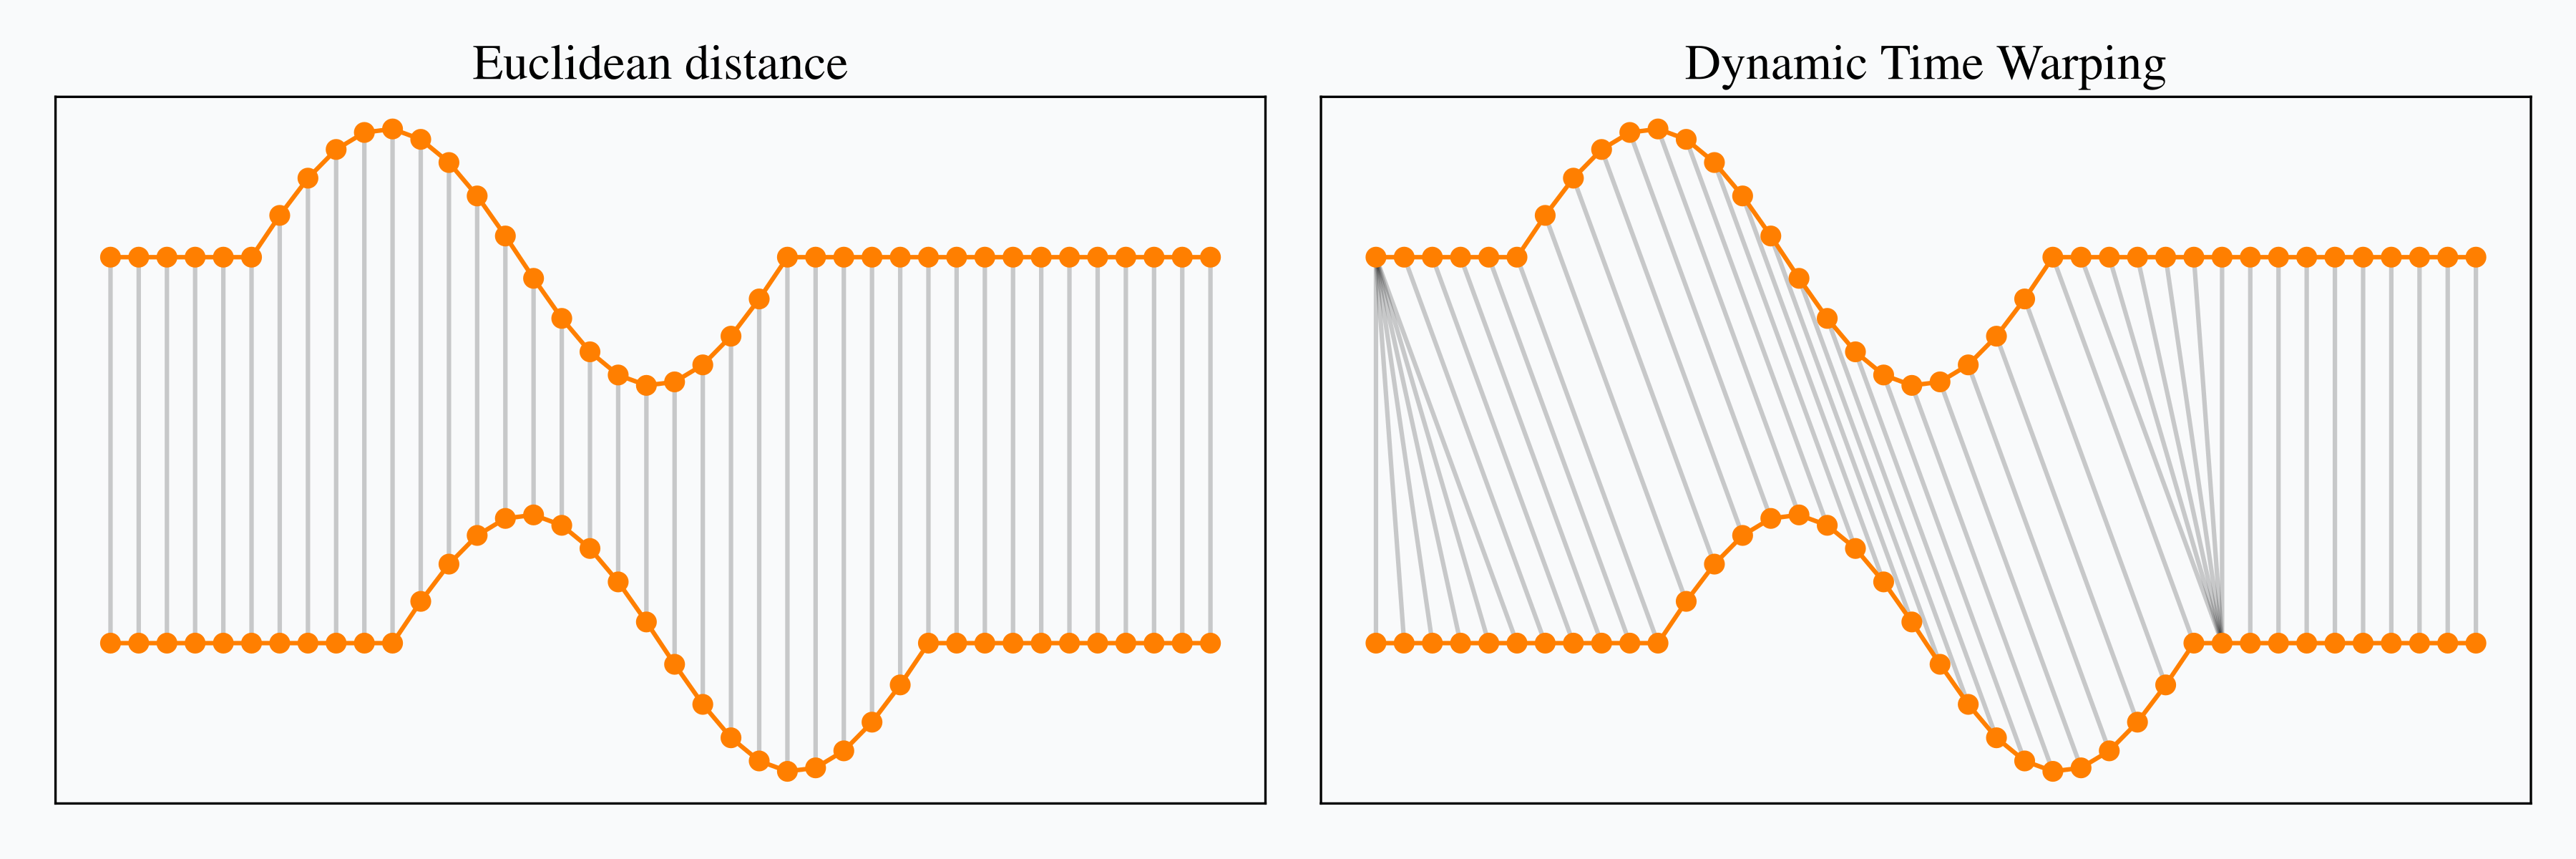
\includegraphics[width=0.8\textwidth]{fig/dtw_vs_euc.png}
    \legend{FONTE: \cite{tavenard.blog.dtw}}
    \label{fig:dtw_intro}
\end{figure}

\section{Vantagens e Desvantagens do DTW}

O DTW apresenta diversas vantagens em relação a outras métricas de distância, como a distância Euclidiana. Entre elas, destacam-se:
\begin{itemize}
    \item \textbf{Robustez a variações de tempo}: O DTW é capaz de lidar com sequências que apresentam variações na velocidade ou no comprimento, permitindo comparações mais precisas.
    \item \textbf{Alinhamento dinâmico}: O DTW encontra o melhor alinhamento entre as sequências, minimizando o custo total de distorção temporal.
    \item \textbf{Versatilidade}: Funciona bem em sinais unidimensionais e multidimensionais, sendo aplicável em diversas áreas como reconhecimento de padrões e análise de séries temporais.
\end{itemize}

No entanto, o DTW também possui desvantagens:
\begin{itemize}
    \item \textbf{Complexidade computacional}: O algoritmo tem complexidade \(O(n \cdot m)\), o que pode ser um limitante para sequências muito longas.
    \item \textbf{Sensibilidade a ruídos}: O DTW pode ser afetado por ruídos nas sequências, o que pode levar a alinhamentos incorretos.
\end{itemize}


\section{Justificativa para o uso do DTW}

Neste trabalho, o DTW foi utilizado por ser uma técnica adequada para comparar sequências que representam características espaciais extraídas de contornos faciais utilizando um algoritmo simples. As curvas resultantes dessas características podem variar em comprimento e forma devido a diferentes condições de iluminação, expressões faciais ou ângulos de captura. O DTW permite alinhar essas curvas de forma dinâmica, possibilitando uma comparação mais precisa entre elas.

Além disso, este trabalho se fundamenta na abordagem proposta por \citet{DTW_LSTM}, que demonstrou a eficácia do uso do algoritmo DTW na comparação da variação das cores dos pixels, obtendo acurácias de 100\%, 94\% e 70\%, conforme as especificidades de cada experimento em tarefas de reconhecimento facial.

Entretanto, uma limitação relevante observada nesse estudo foi o alto custo computacional do DTW, o que compromete sua aplicabilidade em cenários que exigem processamento em tempo real. Embora o tempo exato de execução dos experimentos não tenha sido reportado pelos autores, foi implementado um script com base na proposta do artigo, cujo tempo de execução estimado foi de aproximadamente 10 horas para comparar duas imagens representadas por vetores de dimensão 77.284 (correspondentes às cores dos pixels).

Diante disso, uma das propostas deste trabalho é otimizar o processo de comparação por meio da utilização de curvas suaves representadas por splines, com o objetivo de reduzir a complexidade computacional sem comprometer a acurácia e a eficiência da técnica.



% PARTE DOS RESULTADOS
% ----------------------------------------------------------
%\part{Resultados}
%\input{cap05}

% Finaliza a parte no bookmark do PDF
% para que se inicie o bookmark na raiz
% e adiciona espaço de parte no Sumário
% ----------------------------------------------------------
%\phantompart

% ---
% Conclusão (outro exemplo de capítulo sem numeração e presente no sumário)
% ---
%\chapter*[Conclusão]{Conclusão}
%\addcontentsline{toc}{chapter}{Conclusão}
% ---
%\input{cap06}

% ELEMENTOS PÓS-TEXTUAIS
% ----------------------------------------------------------
\postextual

% Ajuste vertical do titulo de referencias no sumário
% ----------------------------------------------------------
\addtocontents{toc}{\vspace{-6pt}}

% Referências bibliográficas
% ----------------------------------------------------------
% \bibliography{referencias}

\begingroup

\printbibliography[heading=bay,notkeyword= {consulta}, notkeyword={npub-informal}]

\printbibliography [keyword= consulta, title = FONTES DE CONSULTA]
\endgroup

% ----------------------------------------------------------

% Ajuste vertical dos titulos dos capitulos postextuais
% ----------------------------------------------------------
\addtocontents{toc}{\vspace{4pt}}

% Glossário
% ----------------------------------------------------------
% Consulte o manual da classe abntex2 para orientações sobre o glossário.
%
%\glossary

% Apêndices
% ----------------------------------------------------------
\ifthenelse{\equal{\terApendice}{Sim}}
{\begin{apendicesenv}

        % Numeração arábica para os apêndices
        % --------------------------------------------------
        \renewcommand{\thechapter}{\arabic{chapter}}
        % Numeração Alfabética para os apêndices
        % --------------------------------------------------
        % \renewcommand{\thechapter}{\Alph{chapter}} %capitulos  com indicação Alfabética
        %
        % Imprime uma página indicando o início dos apêndices
        % \partapendices

        % Existem várias formas de se colocar anexos.
        % O exemplo abaixo coloca 2 apêndices denominados de 
        % DESENVOLVIMENTO DETALHADO DA PINTURA e 
        % ESCOLHA DO MATERIAL DE IMPRESSÃO:
        % ---
        % --- insere um capítulo que é tratado como um apêndice
        %\chapter{DESENVOLVIMENTO DETALHADO DA PINTURA}
        % 
        %\lipsum[29] % gera um parágrafo
        %
        % --- insere um capítulo que é tratado como um apêndice
        %\chapter{ESCOLHA DO MATERIAL DE IMPRESSÃO}
        % 
        %\lipsum[30] % gera um parágrafo

        % --- Insere o texto do arquivo ap01.tex
        % 
        % --- O conteúdo do arquivo pode ser vários anexos ou um único apêndices.
        %     A vantagem de se utilizar este procedimento é de suprimi-lo
        %     das compilações enquanto se processa o resto do documento.

           % --- insere um capítulo que é tratado como um apêndice
   \label{ap:ap01}
   \chapter{ESCOLHA DO MATERIAL - colocado no apendice}
    
   \lipsum[30] % gera um parágrafo
   \section*{Testes se\c{C}\~aO}

    \lipsum[22] % gera um parágrafo
	
	\chapter{ESCOLHA DO MATERIAL DE IMPRESSÃO- colocado no apendice}
    \lipsum[32] % gera um parágrafo


\end{apendicesenv}
}{}

% Anexos
% ----------------------------------------------------------
\ifthenelse{\equal{\terAnexo}{Sim}}{
\begin{anexosenv}

        % Numeração arábica para os apêndices
        % --------------------------------------------------
        \renewcommand{\thechapter}{\arabic{chapter}}
        % 
        % Numeração Alfabética para os anexos
        % --------------------------------------------------
        % \renewcommand{\thechapter}{\Alph{chapter}} %capitulos  com indicação Alfabética
        % --- Imprime uma página indicando o início dos anexos
        % \partanexos

        % Existem várias formas de se colocar anexos.
        % O exemplo abaixo coloca 2 anexos denominados de 
        % TABELA DE VALORES e GRÁFICOS DE BALANCEMANTO:
        % ---
        % --- insere um capítulo que é tratado como um anexo
        %\chapter{TABELAS DE VALORES}
        % 
        %\lipsum[31] % gera um parágrafo
        %
        % --- insere um capítulo que é tratado como um anexo
        %\chapter{GRÁFICOS DE BALANCEAMENTO}
        % 
        %\lipsum[32] % gera um parágrafo

        % --- Insere o texto do arquivo ax01.tex
        % 
        % --- O conteúdo do arquivo pode ser vários anexos ou um único anexo.
        %     A vantagem de se utilizar este procedimento é de suprimi-lo
        %     das compilações enquanto se processa o resto do documento.

            % --- insere um capítulo que é tratado como um apêndice
   \chapter{anexando ESCOLHA DO MATERIAL}
    
   \lipsum[30] % gera um parágrafo
    \section*{anexando testes secao}
    

\chapter{anexando ESCOLHA DO MATERIAL DE IMPRESSÃO}
    
   \lipsum[32] % gera um parágrafo
 
\end{anexosenv}
}{}

% INDICE REMISSIVO
%---------------------------------------------------------------------
\ifthenelse{\equal{\terIndiceR}{Sim}}{
\phantompart
\printindex
}{}

\end{document}
